\documentclass[twoside,11pt]{report}

% Any additional packages needed should be included after jmlr2e.
% Note that jmlr2e.sty includes epsfig, amssymb, natbib and graphicx,
% and defines many common macros, such as 'proof' and 'example'.
%
% It also sets the bibliographystyle to plainnat; for more information on
% natbib citation styles, see the natbib documentation, a copy of which
% is archived at http://www.jmlr.org/format/natbib.pdf

\usepackage{jmlr2e}
% \usepackage[utf8]{inputenc}%
% \usepackage{tikz}
% \usepackage{cfr-lm}%
\usepackage[T1]{fontenc}%
\usepackage{physics}
\usepackage{amsmath}
% \usepackage{amssymb}
% \usepackage{graphicx}
% \usepackage[margin=3cm]{geometry}
% \usepackage{changepage}
\usepackage{fontspec}
\usepackage{minted}
\usepackage{tcolorbox}
\usepackage{lmodern}
\usepackage{xcolor}
\usepackage{lettrine}
% \usepackage{fontawesome}
\usemintedstyle{perldoc}
\hypersetup{colorlinks=false, pdfborder={0 0 0},  }
\usepackage{fancyhdr}
\usepackage{wrapfig}
\usepackage{adjustbox}
\usepackage{tikz}
% \usepackage{listofitems} % for \readlist to create arrays
\usepackage{caption}
\usepackage[toc,page,header]{appendix}


\newtcbox{\codebox}[1][black]{on line, arc=2pt,colback=#1!10!white,colframe=white, before upper={\rule[-3pt]{0pt}{10pt}},boxrule=1pt, boxsep=0pt,left=2pt,right=2pt,top=1pt,bottom=.5pt}
\newtcbox{\deloppg}[1][black]{on line, arc=2pt,colback=#1!10!white,colframe=white, before upper={\rule[-2pt]{0pt}{0pt}},boxrule=0pt, boxsep=0pt,left=.49\linewidth,right=.49\linewidth,top=4pt,bottom=3pt}


\newcommand\blfootnote[1]{ \begingroup \renewcommand\thefootnote{}\footnote{#1} \addtocounter{footnote}{-1} \endgroup }
% \definecolor{antwhite}{HTML}{323333}
\newcommand{\code}[3][]{\codebox{\mintinline[#1]{#2}{#3}}}



% \setmainfont{FreeSans}
% \setmainfont{SF Pro Display}
% \setmainfont{IBM Plex Sans}
% \setmainfont{TeX Gyre Heros}
% \setmainfont{Inter}
% \setmainfont{Iosevka Quasi}
% \setmainfont{DM Sans}

% \setmonofont{Iosevka Custom Extended}
% \setmonofont{JetBrainsMono Nerd Font}
\setmonofont[Scale=MatchLowercase]{DM Mono}





% Definitions of handy macros can go here

\newcommand{\dataset}{{\cal D}}
\newcommand{\fracpartial}[2]{\frac{\partial #1}{\partial  #2}}

% Heading arguments are {volume}{year}{pages}{submitted}{published}{author-full-names}

% \jmlrheading{1}{2000}{1-48}{4/00}{10/00}{https://github.com/bragewiseth/MachineLearningProjects}

% Short headings should be running head and authors last names

\ShortHeadings{\url{https://github.com/bragewiseth/MachineLearningProjects}}{\url{https://github.com/bragewiseth/MachineLearningProjects}}
\firstpageno{1}



\title{{\huge Project 2}}
\author{\name Brage W. \email bragewi@ifi.uio.no\\
    \name Felix C. H.  \email felixch@ifi.uio.no \\
\name Eirik B. J. \email eiribja@ifi.uio.no}
\date{\today}											% Date
\makeatletter






% \date{\today}

\usepackage{hyperref}
\begin{document}

%%%%%%%%%%%%%%%%%%%%%%%%%%%%%%%%%%%%%%%%%%%%%%%%%%%%%%%%%%%%%%%%%%%%%%%%%%%%%%%%%%%%%%%%%

\begin{titlepage}
    \centering
    \vspace*{0.5 cm}
    
\includegraphics[scale = 0.75]{uio.jpg}\\[1.0 cm]	% University Logo
    \textsc{\LARGE University of Oslo}\\[2.0 cm]	    % University Name
    \textsc{\Large FYS-STK3155}\\[0.5 cm]				% Course Code
    \rule{\linewidth}{0.2 mm} \\[0.4 cm]
    { \huge \bfseries \@title}\\
    \rule{\linewidth}{0.2 mm} \\[1.5 cm]

    \begin{minipage}{0.4\textwidth}
        \begin{flushleft} \normalsize
            Brage Wiseth\\
            Felix Cameren Heyerdahl\\
            Eirik Bjørnson Jahr\\
        \end{flushleft}
    \end{minipage}~
    \begin{minipage}{0.4\textwidth}
        \begin{flushright} \normalsize
            \textsc{
                bragewi@ifi.uio.no\\
                felixch@ifi.uio.no\\
                eiribja@ifi.uio.no\\
            }
        \end{flushright}

    \end{minipage}\\[2 cm]
    \@date\\
    \vspace*{25mm}
    \urlstyle{rm}
    \textsc{\url{https://github.com/bragewiseth/MachineLearningProjects}}







\end{titlepage}
\nocite{*}
% \maketitle
\newpage
\tableofcontents
\newpage




\begin{abstract}%   <- trailing '%' for backward compatibility of .sty file
    \lettrine{I}{}n this paper, we investigate the viability of using neural networks to solve
    classification problems. Specifically, we compare the performance of neural networks
    with that of traditional logistic regression models. There are many real world applications
    and problems that require us to correctly differntiae between some classes. For example, in the field of
    cancer research, it is often necessary to classify a tumor as either benign or malignant. this
    can be done by extracting a set of features from the tumor and differentiating between the two
    classes based on how different classes posess slight variations across the features. 
    However, some features may be more or less equal for both classes, and the
    amount of features may be large. These two factors may make it difficult for a human to classify the tumor.
    By using a neural network, we achieved a classification accuracy of 98\% on the Wisconsin breast cancer
    dataset. With logistic regression, we achieved an accuracy of 98\%. Comparing that with SKLearns model
    we achieved an accuracy of 96\%.
    In addition to classification, we also investigated the use of neural networks for regression problems
    see Appendix~\hyperref[app:appendixA]{A}.
    We found that neural networks are able to approximate the Franke function with a mean squared error of
    0.0001. This is comparable to the results we achieved with linear regression. However, we found that
    neural networks are much more sensitive to the choice of learning rate and number of epochs. We also
    found that neural networks are much more computationally expensive than linear regression.\\
\end{abstract}
\begin{keywords}
    Regression, Classification, Neural Networks
\end{keywords}








\addcontentsline{toc}{section}{Introduction}
\section*{Introduction}



In project 1\cite{MachineLearningProjects_2023}, we found that 
we can fit lines or even polynimals that approximate the distribution of our data by solving an nice analytical expression for the optimal parameters $\beta$. We can in principle approximate 
any function with a polynomial, if we give ourselves infinite degrees of freedom. This is great but there are several
limitations to this approach. First of all, we can not give ourselves infinite degrees of freedom, believe it or not.
Secondly, what if we don't want to find a polynimal but rather classify our data into some classes?\\

\noindent
To tackle classification we can use \emph{logistic regression}, that is, first regression and then clamp the output to a binary value
(for the bianry case). We can do this with an activation function like the sigmoid function
\footnote{The sigmoid function does not output a binary value, but a value between 0 and 1. 
    We can then set a threshold, for example 0.5, and say that if the output is above the threshold, 
    we classify it as 1, and if it is below, we classify it as 0. We can interpret the output as the 
probability of the data point being 1.}
or the heaviside function. However the first problem
still remains, we want to approximate any function, but don't want to use an infinite taylor series. 
We need a different approach.
Instead of finding a single high degree polynimial, we can try to glue together a bunch of smaller line segments.
For this we can use a \emph{neural network}.
As it turns out, the framework for neural networks is very similar to the framework for logistic regression.
Neural networks can be interpeted as several logistic regression models glued together, which is exactly what we wanted!
Another huge benefit of this is that we can use the same code
For both logistic and linear regression as well as neural networks.
This sounds great, but by introducing activation functions we lose the nice analytical expression,
so we can't use the same matrix inversion approach as before.\\
So how do we learn?


\noindent
\textbf{Gradient Decent}:\\ 
In this section we will discuss the gradient decent algorithm and how it can be used to
optimize the parameters of a model.\\
\textbf{Data}: \\
In this section we will discuss the data we will be using in this project.\\
\textbf{Results}:\\
In this section we will discuss the results we achieved with our models.\\
\textbf{Conclusion}:\\
In this section we will discuss the results we achieved with our models.\\

\section{Gradient Descent}
\label{sec:GD}

Gradient descent is an iterative optimization algorithm for finding the minimum of a function.
The idea is to take steps in the direction of the negative gradient of the function. It is
verry similar to the Newton-Raphson method for finding roots of a polynimal,
but instead of using the second derivative, we use the first derivative.

optimizers

stocastic


\subsection{Backpropagation and Chain Rule}
\label{sec:backpropagation}

Calculating derivatives is the bread and butter of machine learning. For the simpelest models, like linear regression,
the derivatives are relatively easy and straight forward to calculate. We simply take the derivative of the cost function
with respect to our parameters. However, for more complex models, like neural networks, the derivatives 
are not so easy to calculate.
When the loss function is a composition of several functions, we need to invoke the chain rule. 

\begin{figure}[!h]
    \begin{center}
        Forward\\
        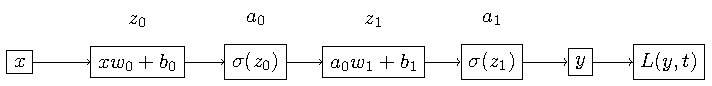
\includegraphics[width=\textwidth]{tikzfigures/forward.pdf}\\
    \end{center}
    If we want to calculate the derivative of the loss function with respect to $w_0$,
    we must go trough all the functions in the chain and calculate the derivative of 
    each function with respect to the next function.
    \begin{center}
        Backwards\\
        \hspace{1cm}
        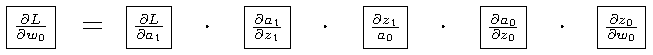
\includegraphics[width=\textwidth]{tikzfigures/backwards.pdf}
    \end{center}
    \caption{chain rule}\label{fig:chainrule}
\end{figure}




\section{Neural Networks}
\label{sec:NN}


\begin{figure}
    \begin{center}
        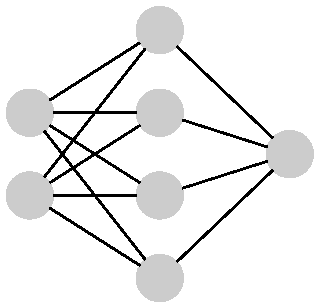
\includegraphics[width=0.4\textwidth]{tikzfigures/nn.pdf}
    \end{center}
    \caption{A model of a neural network with one hidden layer consisting of four nodes}\label{fig:nn}
    \cite{neutelings_tikzcode}
\end{figure}
\begin{figure}
    \begin{center}
        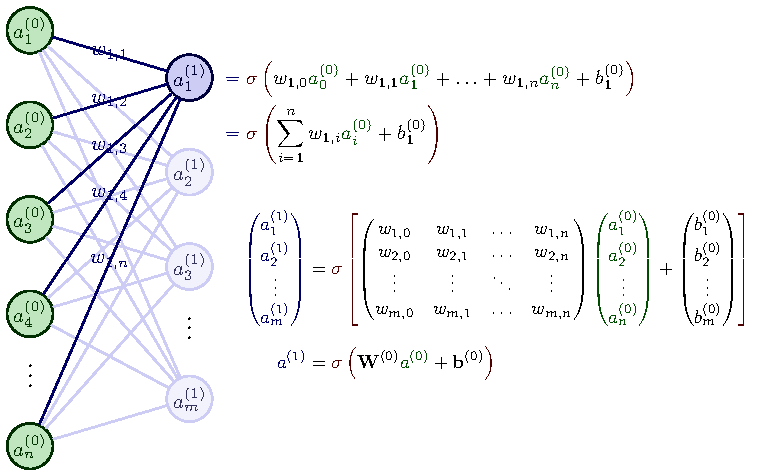
\includegraphics[width=\textwidth]{tikzfigures/nnActivation.pdf}
    \end{center}
    \caption{}\label{fig:nn_math}
    \cite{neutelings_tikzcode}
\end{figure}


With backpropagation we have a way to calculate the derivatives of the loss function with 
respect to the parameters. This allows us to train our neural network. 
with one layer the network becomes a linear regression model. $y = x_0w_0 + x_1w_1 + x_2w_2 + ... + x_nw_n + b_0$ 
with a activation function at the end we can make it into a logistig regression model.
This makes it very convenient to use the same code for both linear and logistic regression as well as for 
larger neural networks with hidden layers, by simply swapping out the different parts.


activation functions




\section{Data}
\label{sec:data}
for classification we will be using the Wisconsin breast cancer dataset [cite here]. This dataset contains 569 data points
with 30 features each. The features are computed from a digitized image of a fine needle aspirate (FNA) of a breast mass.
They describe characteristics of the cell nuclei present in the image. The features are computed for each cell nucleus:
radius, texture, perimeter, area, smoothness, compactness, concavity, concave points, symmetry, fractal dimension.
The mean, standard error and "worst" or largest (mean of the three largest values) of these features were computed for each image,
resulting in 30 features. For example, field 3 is Mean Radius, field 13 is Radius SE, field 23 is Worst Radius.
All feature values are recoded with four significant digits. Missing attribute values: none.
Class distribution: 357 benign, 212 malignant

malignant = cancer.data[cancer.target==0]
benign = cancer.data[cancer.target==1]

the goal is to classify the tumors as either benign or malignant based on the features.
a positive result means that the tumor is malignant, and a negative result means that the tumor is benign.
in other words, we want to find the cases of cancer and classify them as positive

\begin{figure}
    \begin{center}
        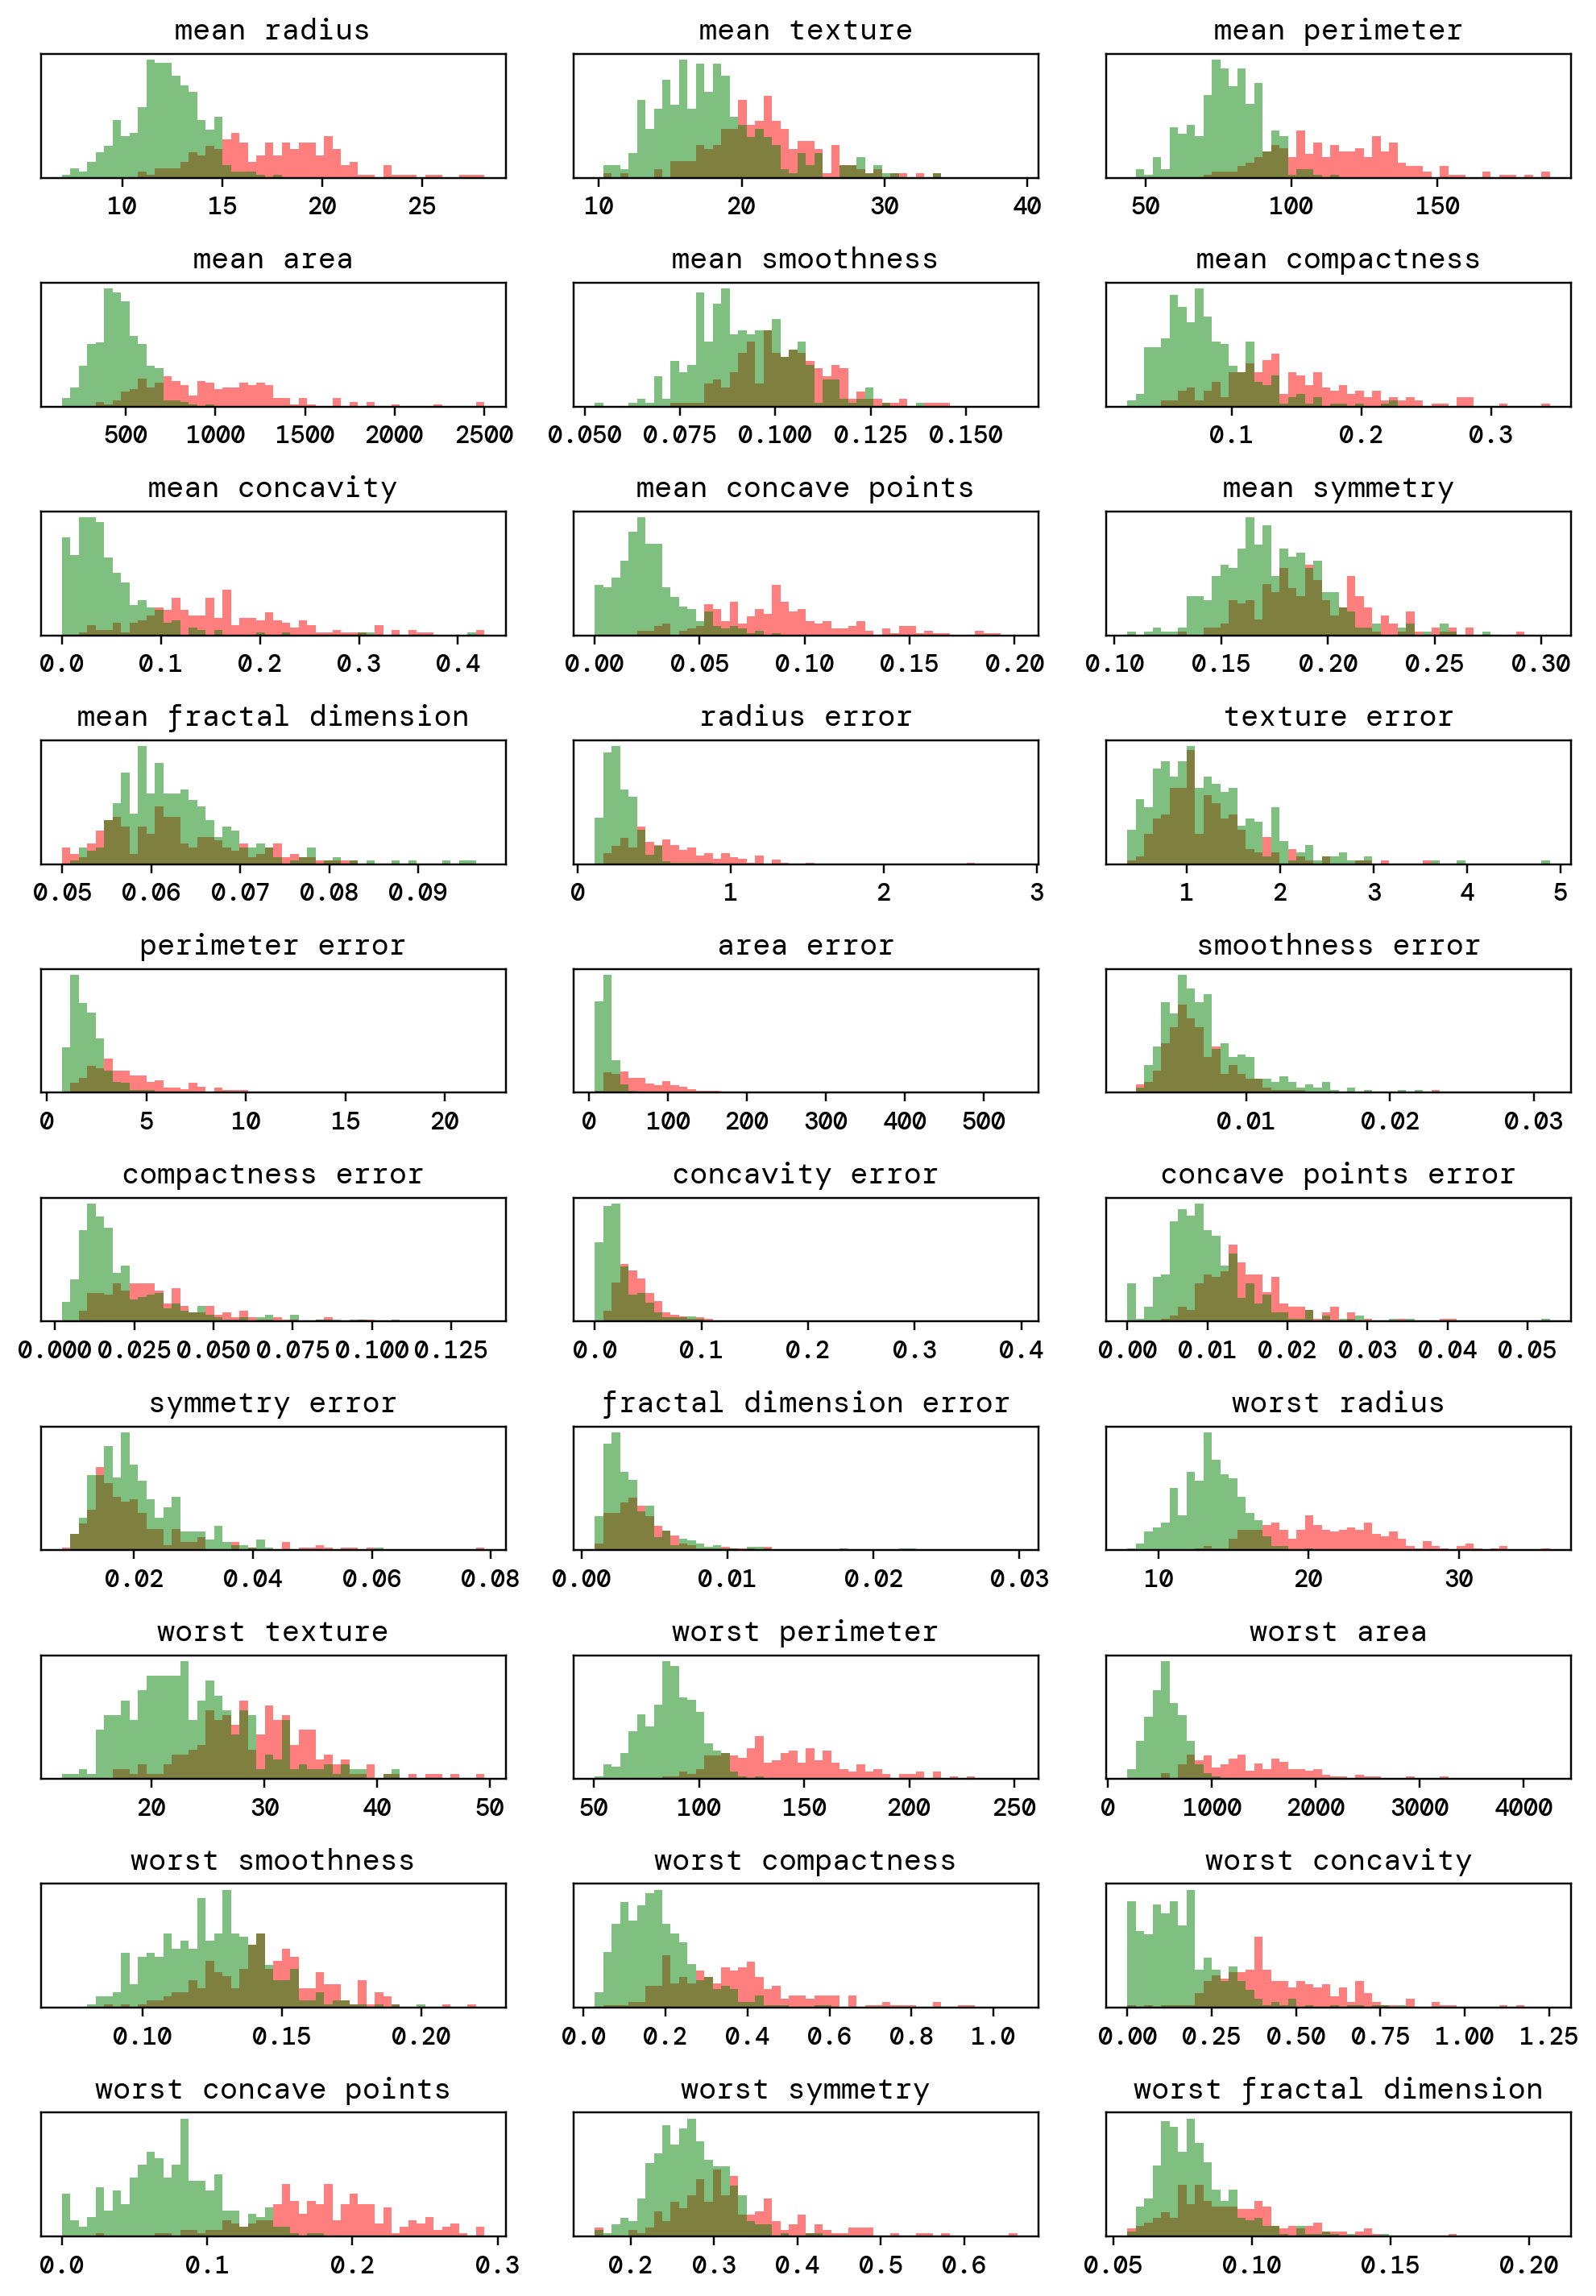
\includegraphics[width=\textwidth]{../runsAndFigures/feature_histogram.png}
    \end{center}
    \caption{Feature histogram}\label{fig:feature_histogram}
\end{figure}

\begin{figure}
    \begin{center}
        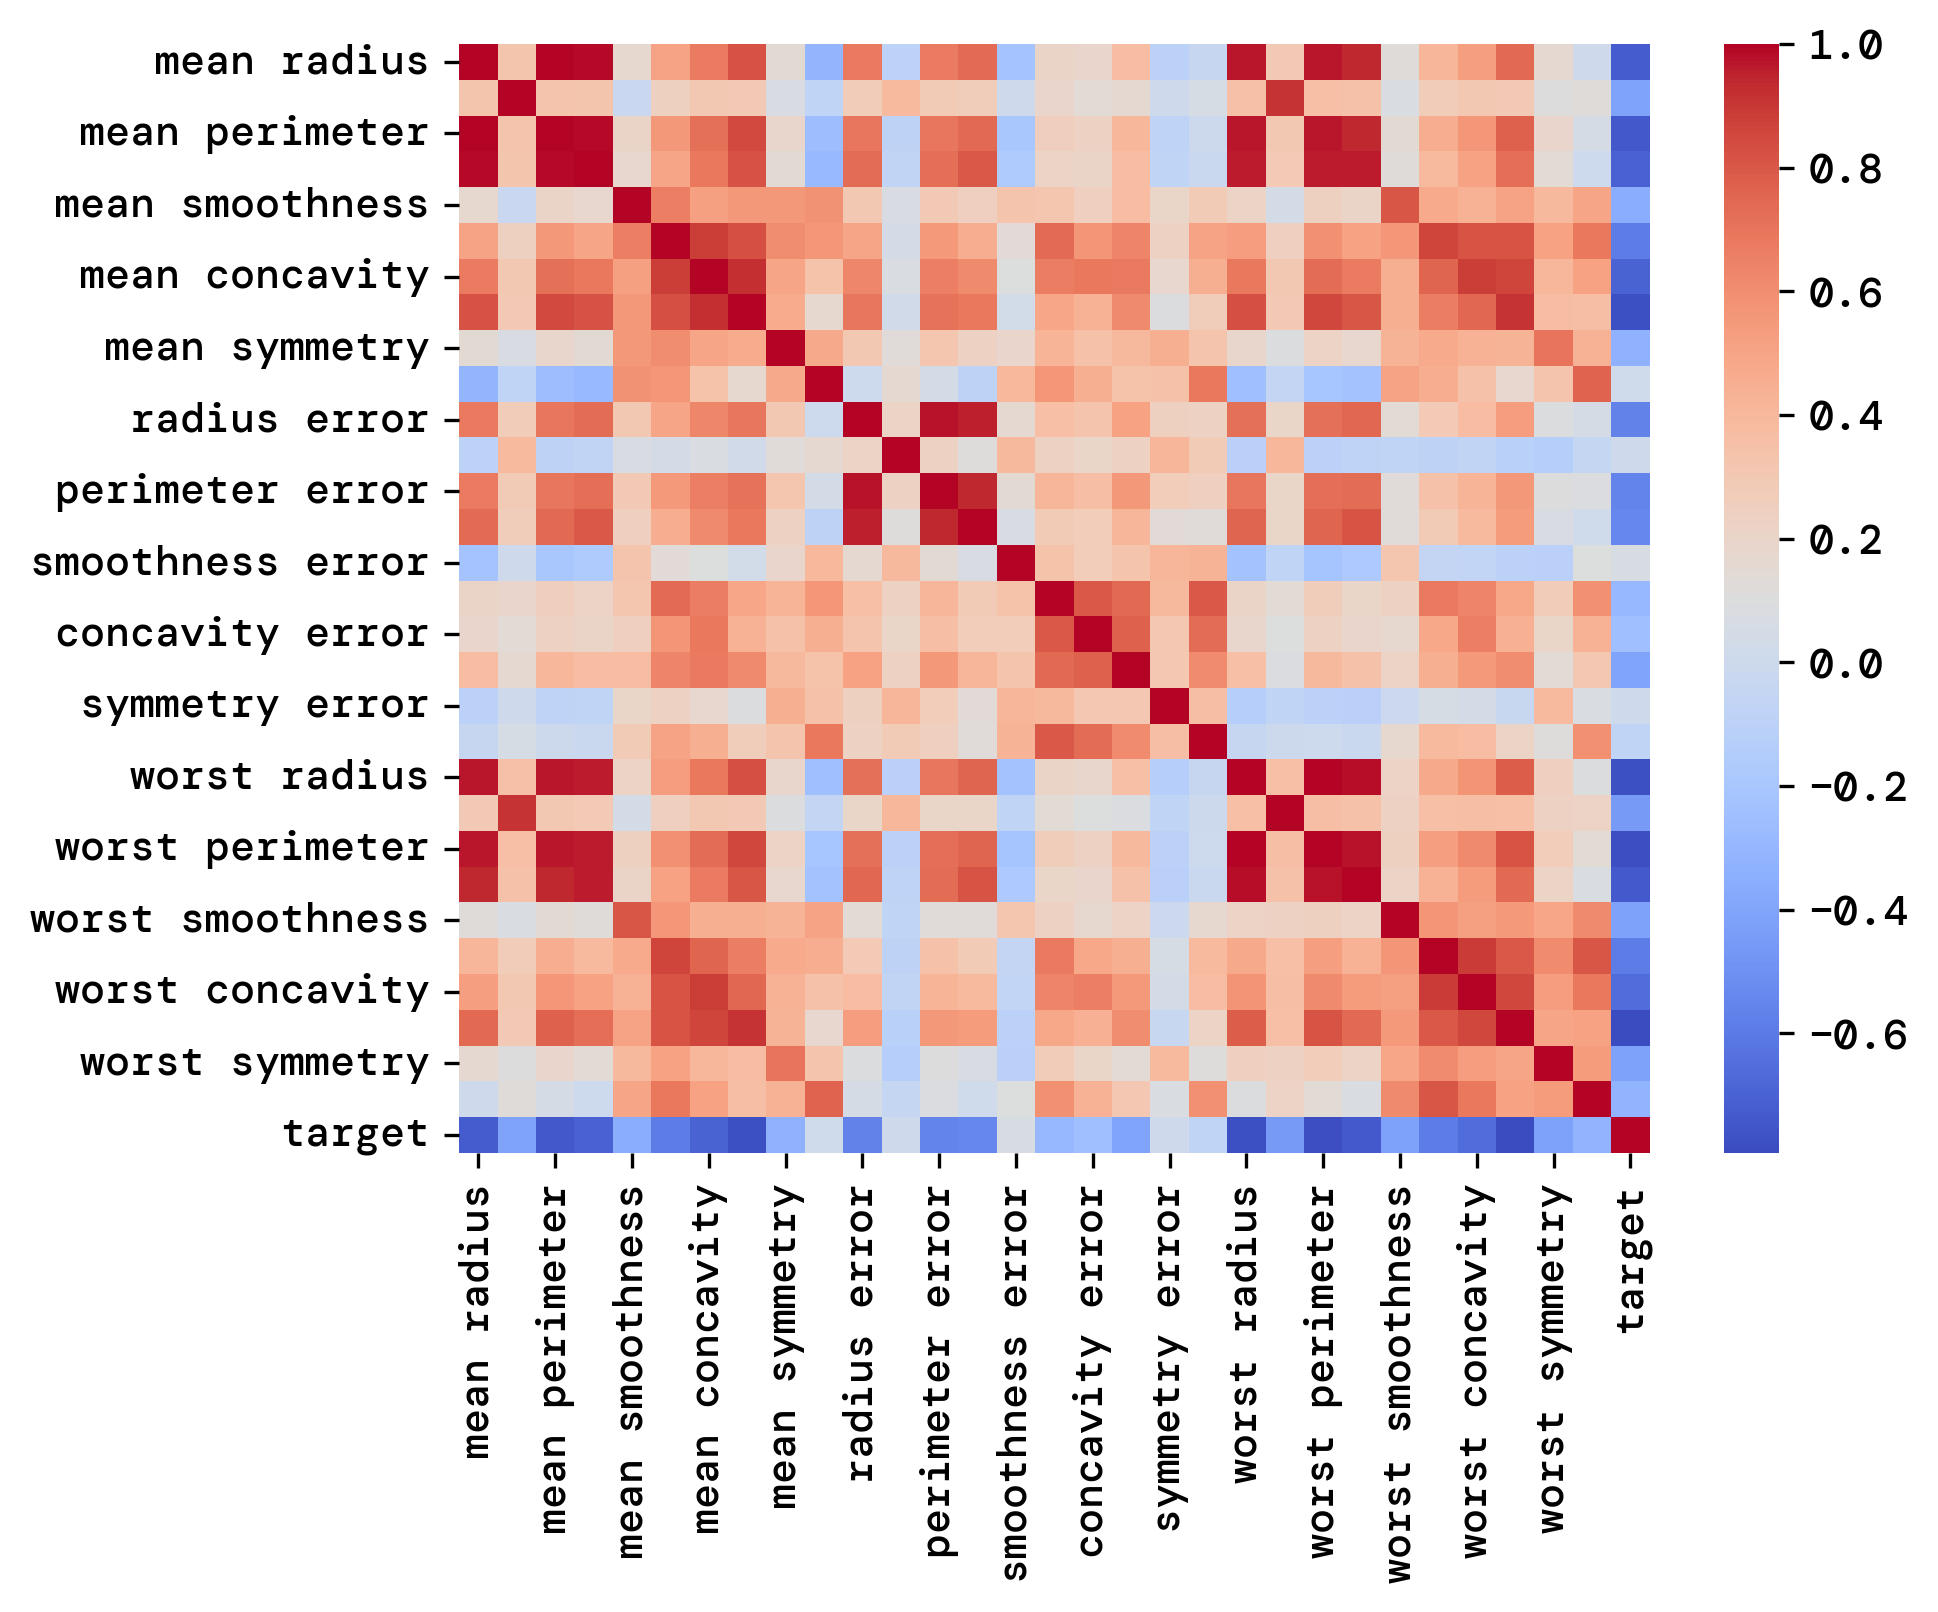
\includegraphics[width=\textwidth]{../runsAndFigures/feature_correlation.png}
    \end{center}
    \caption{Feature correlation. Gives us an idea of the redundancy of the features.
        Only every other features is annotated but you can infer the missing lables 
    from Figure~\ref{fig:feature_histogram}}\label{fig:feature_correlation}
\end{figure}




\section{Results and Analysis}
\label{sec:resultsdiscussion}

For classification we use the cross entropy loss function. 
We tune the hyperparameters in a grid searches with a maximum
of two dimensions. As we find the optimal hyperparameters, we use the same optimal hyperparameters for the next grid search.

some of the hyperparameters are more dependent on each other than others. For example, the learning rate and the number of epochs
the batch size and the learning rate. We can therefore not tune these hyperparameters independently. We must first find the optimal

due to our limited time and computational resources we have not been able to do a full grid search for all hyperparameters. 

\subsection{Hyperparameters}
\label{sec:hyperparameters}
epochs found to be 200 

when training for batch size we had to decrease the optimal learning rate due to unstable results for smaller batches

\begin{figure}[!ht]
    \begin{minipage}[t]{0.5\textwidth - 1mm}
        \begin{center}
            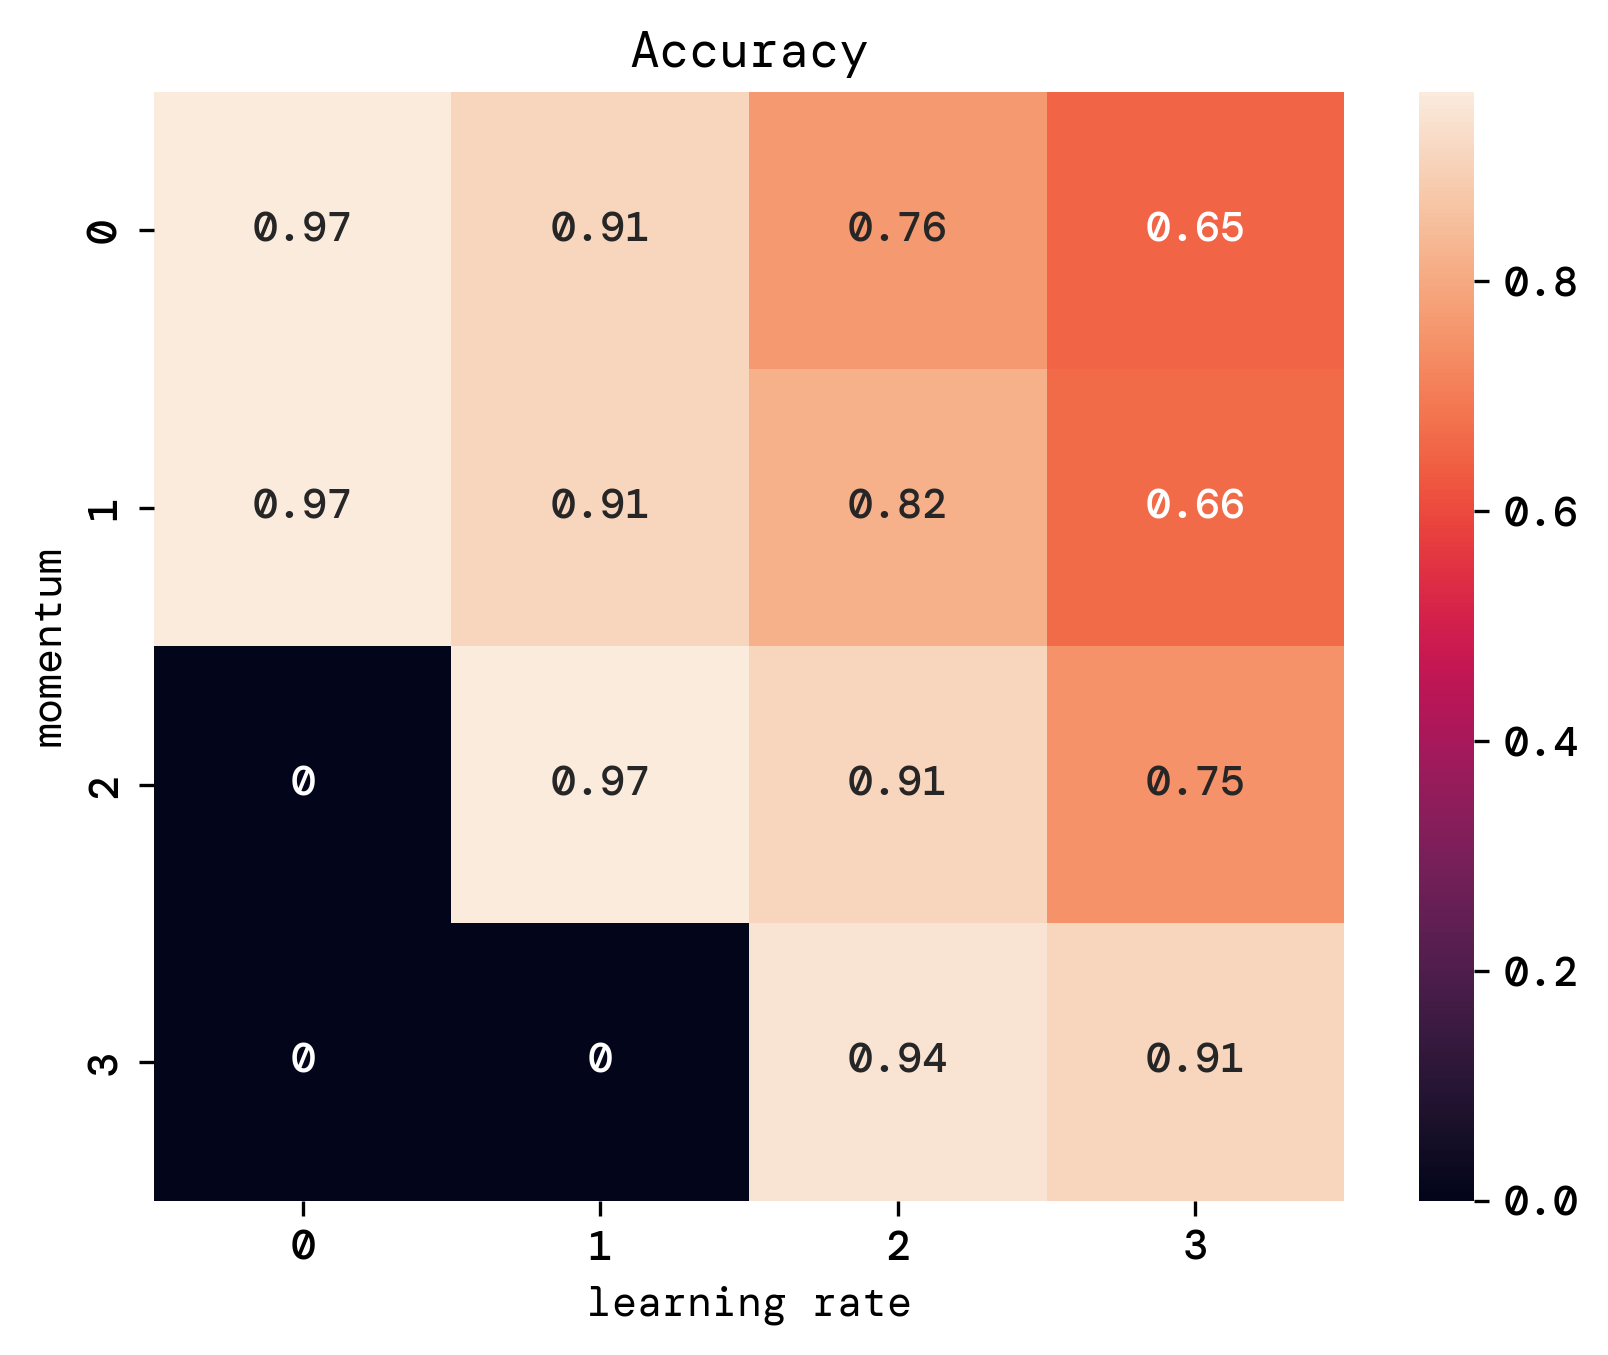
\includegraphics[width=\textwidth]{../runsAndFigures/accuracy_lr_gamma.png}
        \end{center}
        \caption{In this case havving momentum seems to be beneficial. We maxes out our testing range and found that 0.9 was the best value for momentum. momentum allows a higher learning rate}\label{fig:accuracy_lr_gamma}
    \end{minipage}
    \hspace{2mm}
    \begin{minipage}[t]{0.5\textwidth - 1mm}
        \begin{center}
            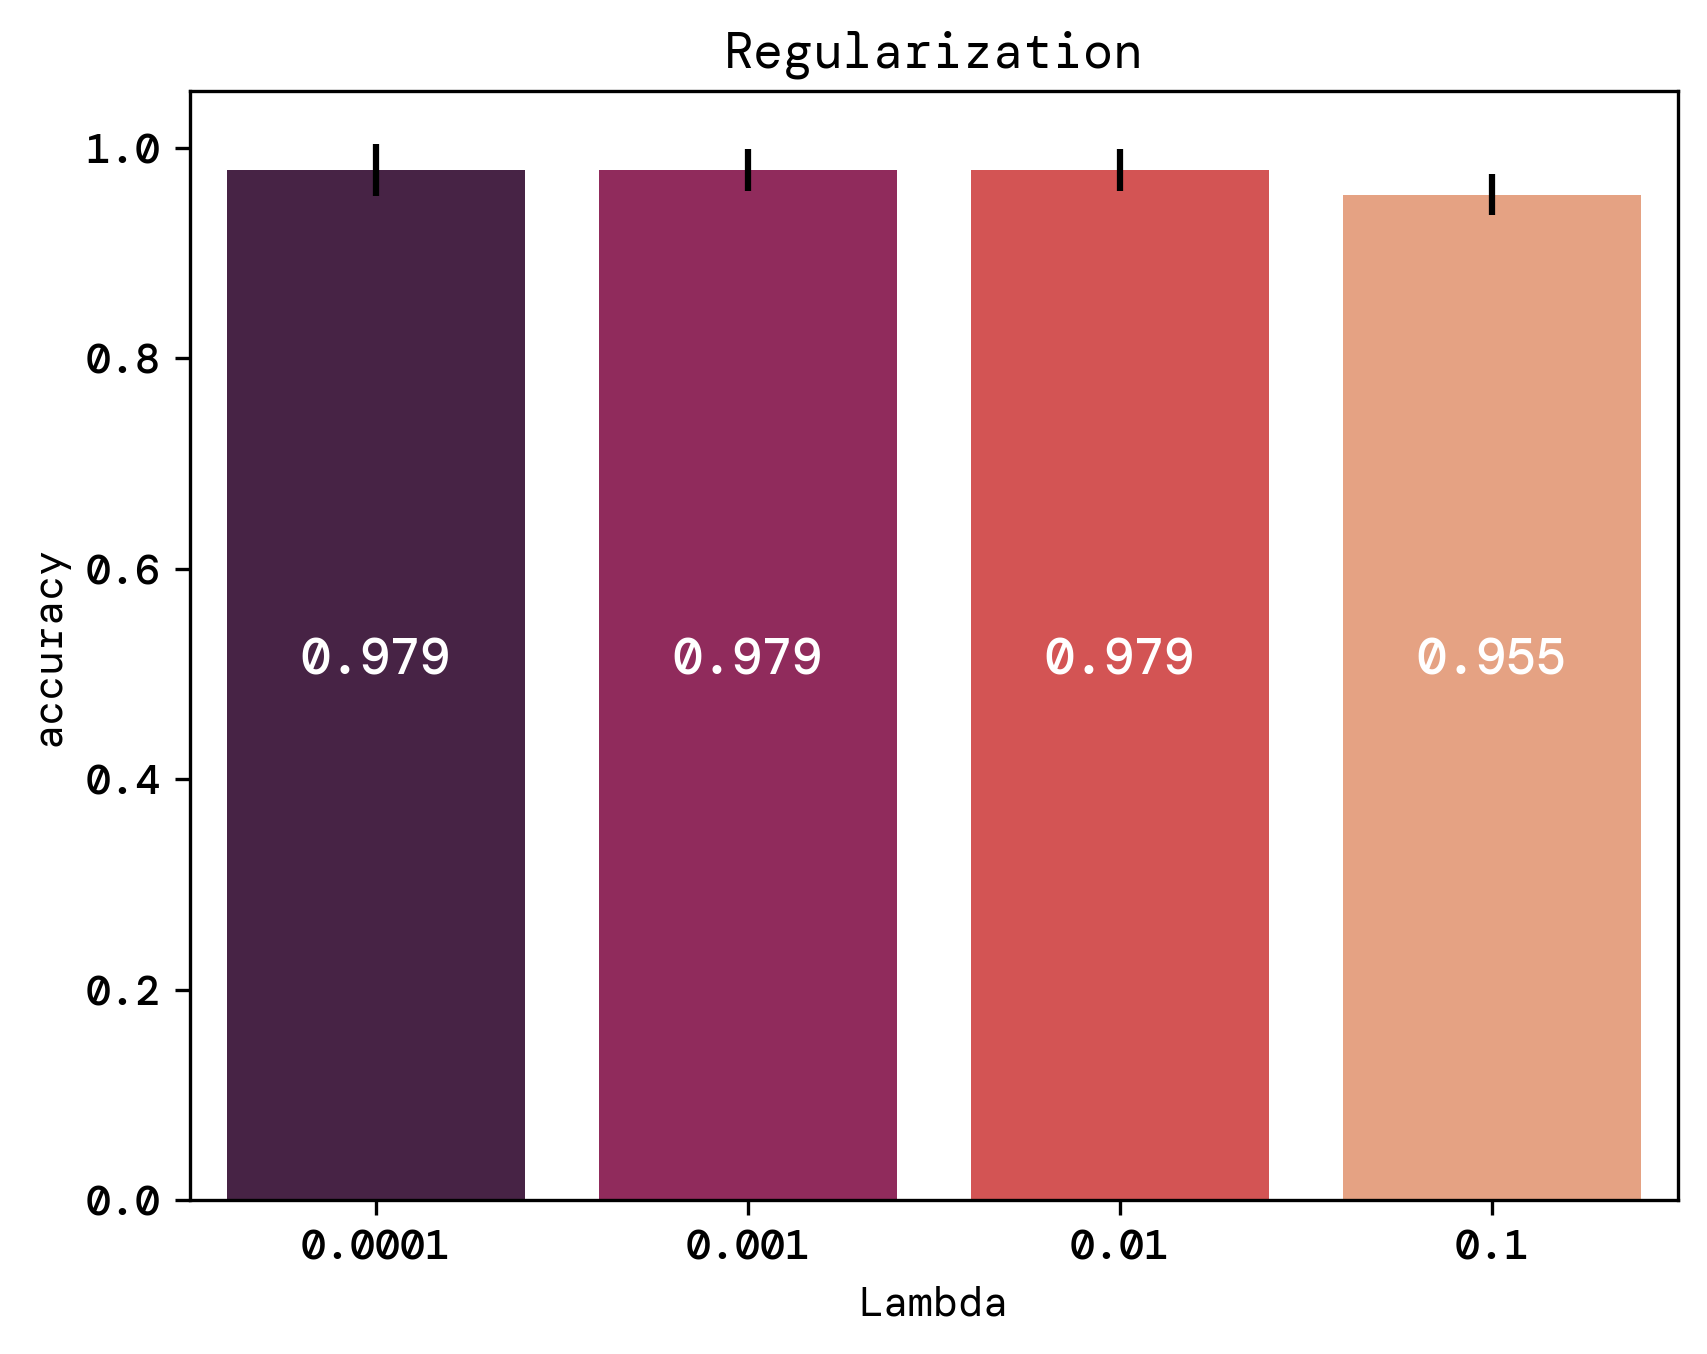
\includegraphics[width=\textwidth]{../runsAndFigures/accuracy_alpha.png}
        \end{center}
        \caption{Introduction regualarization does not seem to yield any benefits, in fact
        having too much regualarization shunts performance}\label{fig:accuracy_aplha}
    \end{minipage}
\end{figure}


\begin{figure}[!ht]
    \begin{minipage}[t]{0.5\textwidth - 1mm}
        \begin{center}
            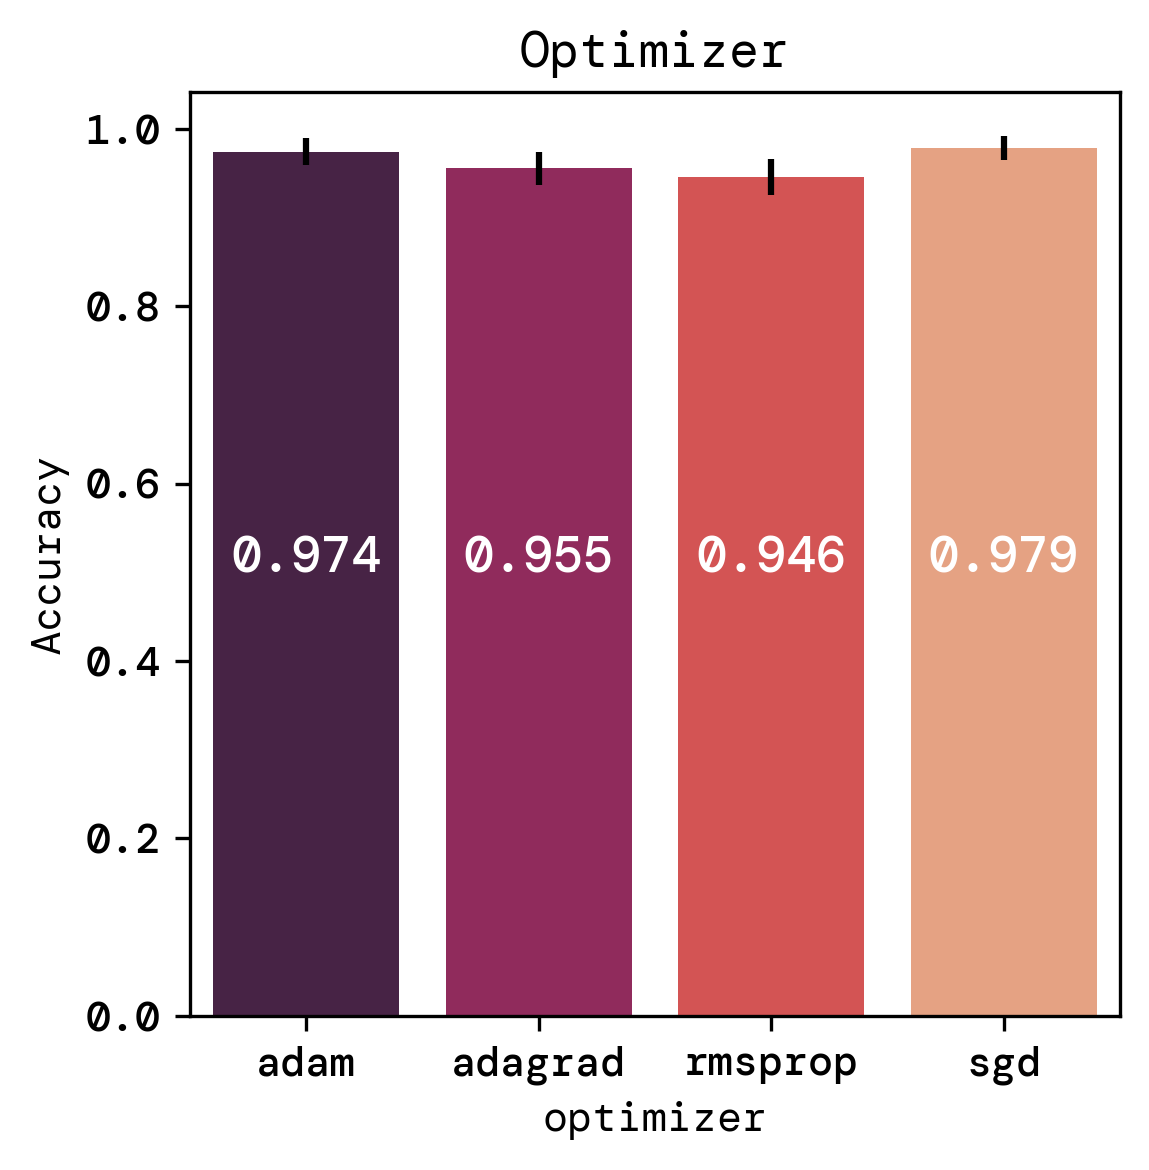
\includegraphics[width=\textwidth]{../runsAndFigures/accuracy_optimizer.png}
        \end{center}
        \caption{In this case havving momentum seems to be beneficial. We maxes out our testing range and found that 0.9 was the best value for momentum. momentum allows a higher learning rate}\label{fig:accuracy_optimizer}
    \end{minipage}
    \hspace{2mm}
    \begin{minipage}[t]{0.5\textwidth - 1mm}
        \begin{center}
            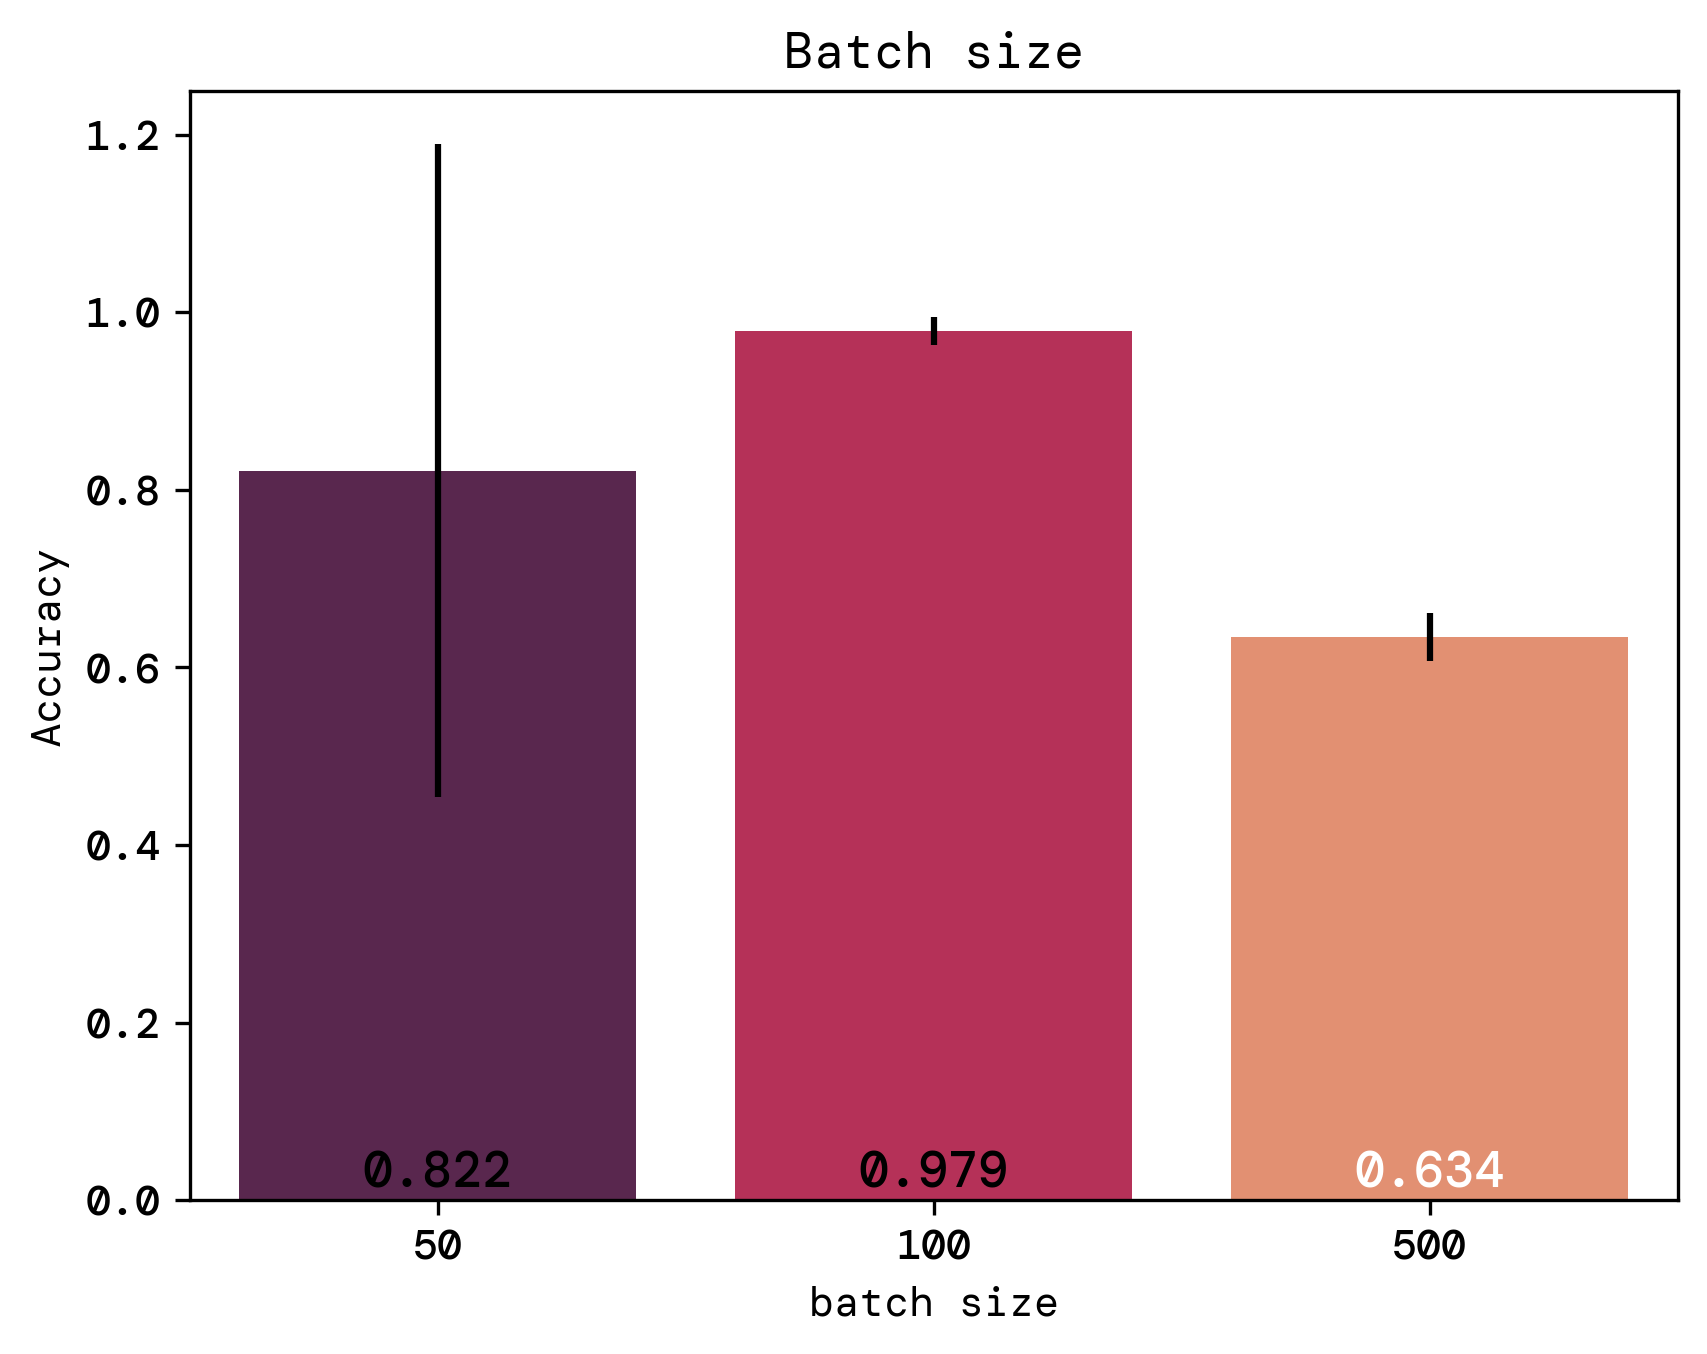
\includegraphics[width=\textwidth]{../runsAndFigures/accuracy_batch.png}
        \end{center}
        \caption{Introduction regualarization does not seem to yield any benefits, in fact
        having too much regualarization shunts performance}\label{fig:accuracy_aplha}
    \end{minipage}
\end{figure}


\begin{figure}[!ht]
    \begin{minipage}[t]{0.5\textwidth - 1mm}
        \begin{center}
            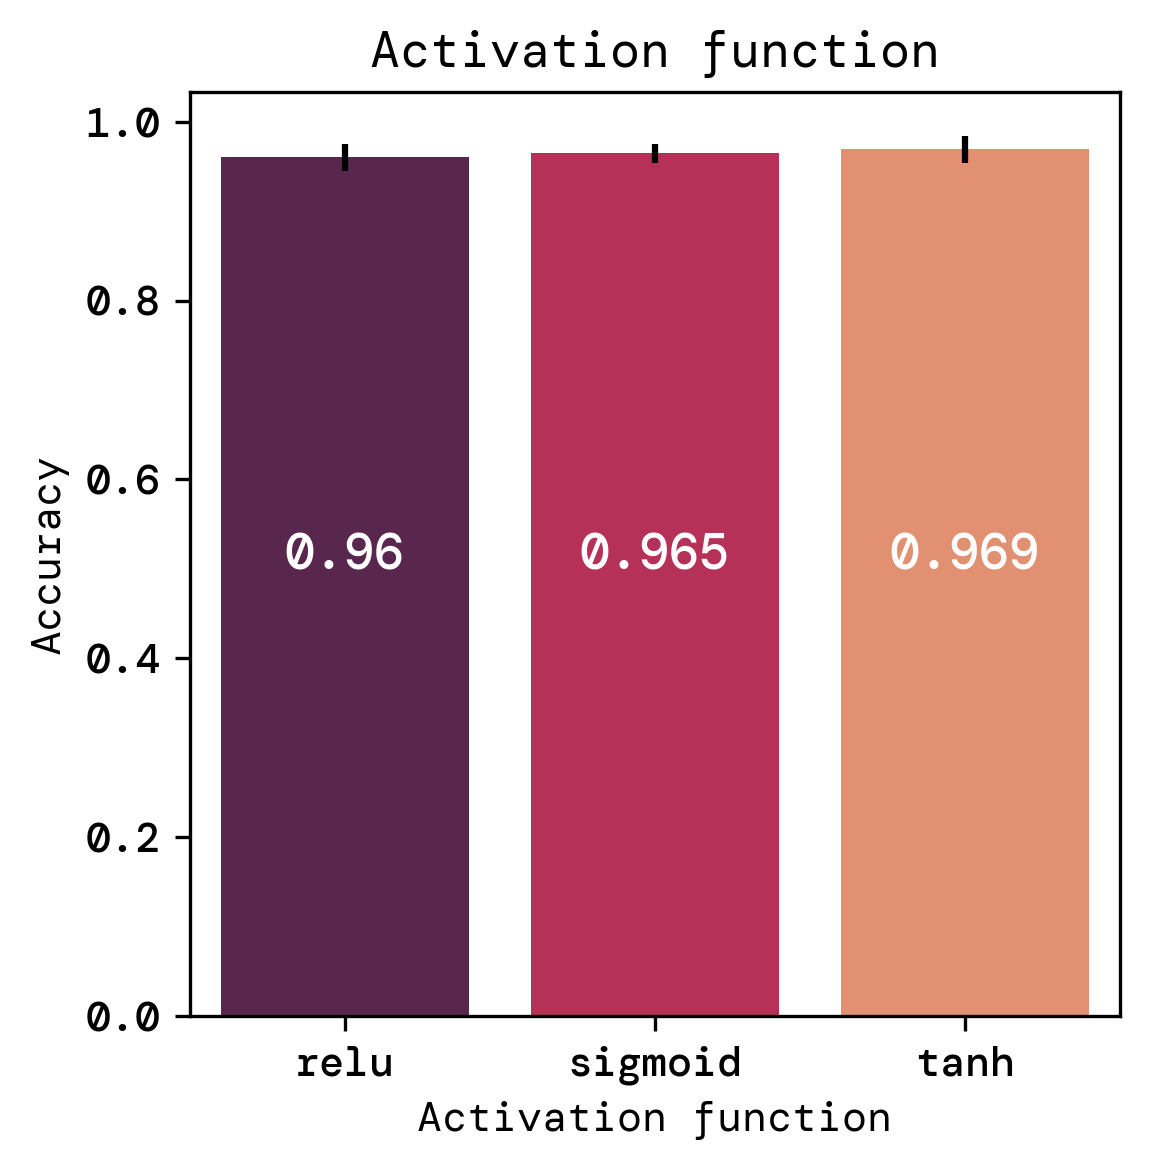
\includegraphics[width=\textwidth]{../runsAndFigures/accuracy_activ.png}
        \end{center}
        \caption{In this case havving momentum seems to be beneficial. We maxes out our testing range and found that 0.9 was the best value for momentum. momentum allows a higher learning rate}\label{fig:accuracy_optimizer}
    \end{minipage}
    \hspace{2mm}
    \begin{minipage}[t]{0.5\textwidth - 1mm}
        \begin{center}
            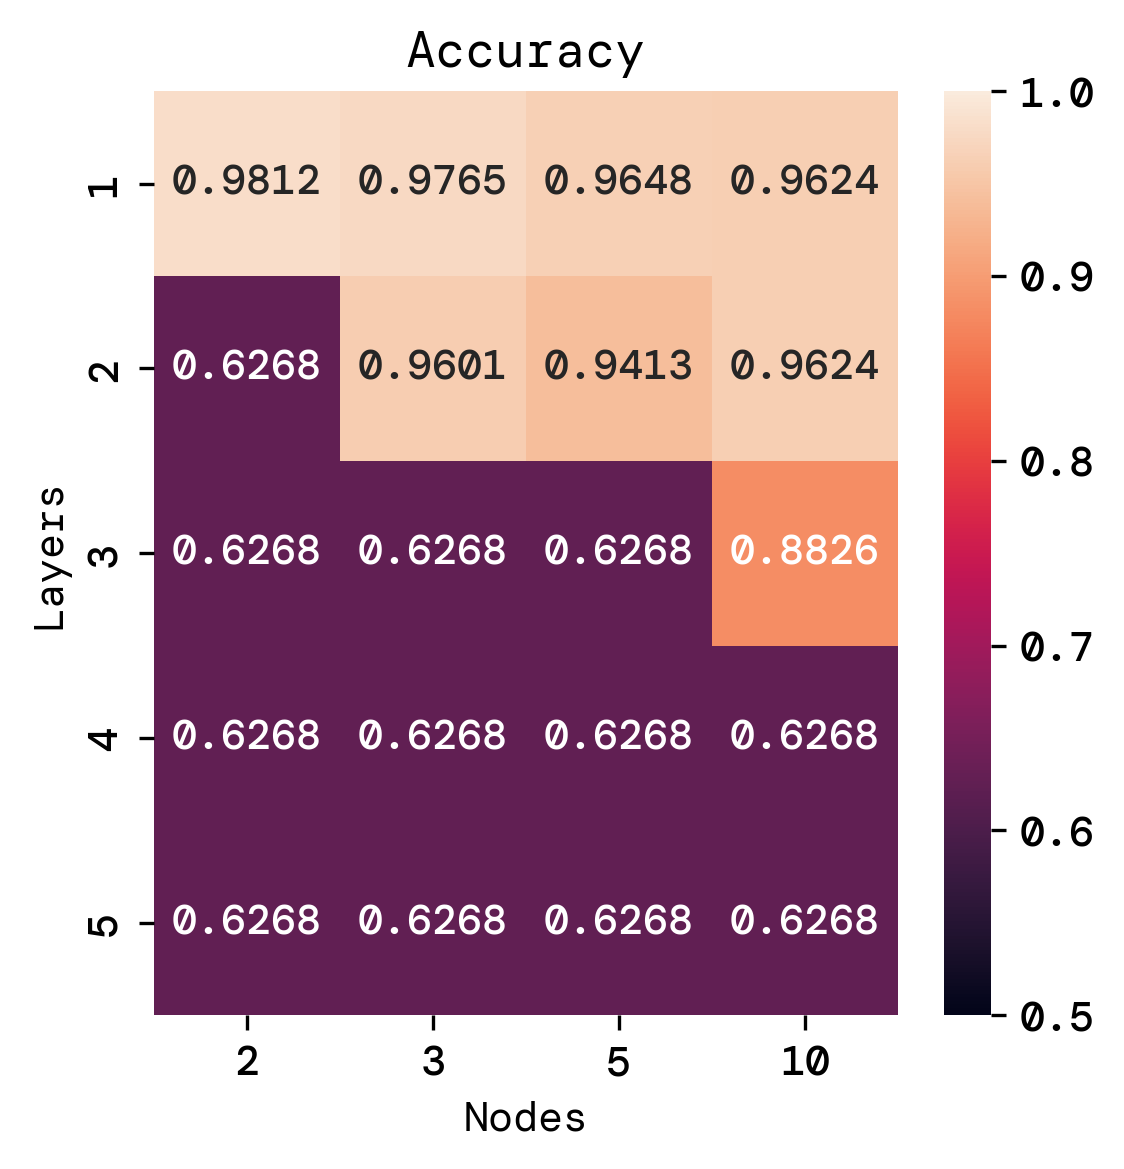
\includegraphics[width=\textwidth]{../runsAndFigures/accuracy_layers_nodes.png}
        \end{center}
        \caption{Introduction regualarization does not seem to yield any benefits, in fact
        having too much regualarization shunts performance}\label{fig:accuracy_aplha}
    \end{minipage}
\end{figure}



\subsection{Final Evaluation and Comparisons}
\label{sec:comparisons}




\section{Conclusion}
\label{sec:conclusion}


Lorem ipsum dolor sit amet, officia excepteur ex fugiat reprehenderit enim labore culpa sint ad nisi Lorem pariatur mollit ex esse exercitation amet. Nisi anim cupidatat excepteur officia. Reprehenderit nostrud nostrud ipsum Lorem est aliquip amet voluptate voluptate dolor minim nulla est proident. Nostrud officia pariatur ut officia. Sit irure elit esse ea nulla sunt ex occaecat reprehenderit commodo officia dolor Lorem duis laboris cupidatat officia voluptate. Culpa proident adipisicing id nulla nisi laboris ex in Lorem sunt duis officia eiusmod. Aliqua reprehenderit commodo ex non excepteur duis sunt velit enim. Voluptate laboris sint cupidatat ullamco ut ea consectetur et est culpa et culpa duis.




















% \acks{}


\clearpage % Start a new page before the appendix
% \pagenumbering{arabic} % Switch to Arabic page numbering (1, 2, 3, ...)
% \setcounter{page}{1} % Set the page number to 1
% \renewcommand{\thepage}{A-\arabic{page}} % Redefine the page numbering format

\appendix
\renewcommand{\theHchapter}{appendix\Alph{chapter}}
\renewcommand{\theHsection}{appendix\thesection}

\phantomsection
\addcontentsline{toc}{chapter}{Appendix}


\chapter*{Appendix A}
\label{app:appendixA}


\section{Regression with Neural Networks}
\label{sec:regression}


\section*{Data}

For regression we will be using perlin noise to generate our dataset 

\begin{figure}
    \begin{center}
        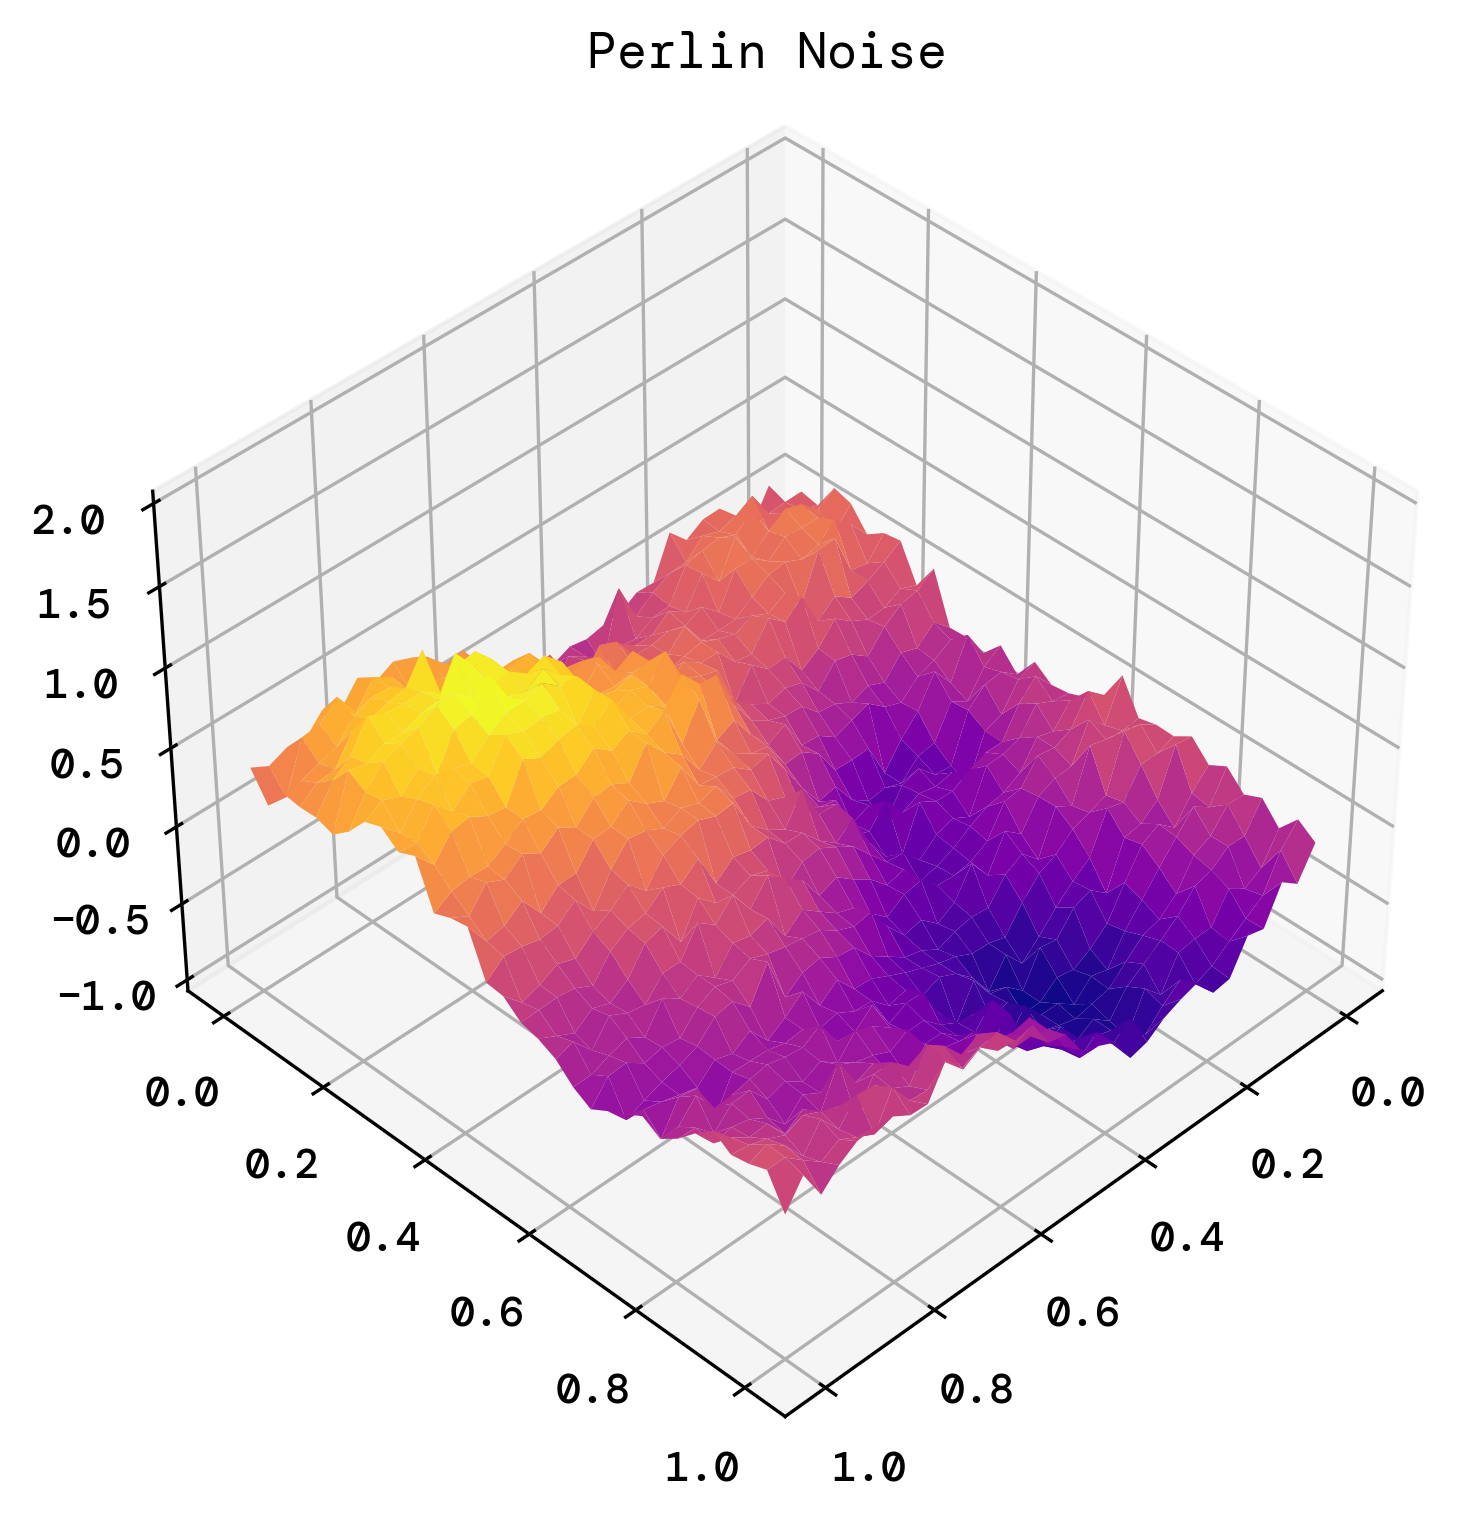
\includegraphics[width=0.5\textwidth]{../runsAndFigures/perlinNoise.png}
    \end{center}
    \caption{}\label{fig:perlin}
\end{figure}

Solving a regression problem with linear regression and neural networks using gradient optimization.



\section*{Results and Analysis}
\label{sec:resultsdiscussion2}




\subsection*{Hyperparameters}
\label{sec:hyperparameters2}


\begin{figure}[!ht]
    \begin{minipage}[t]{0.49\textwidth}
        \begin{center}
            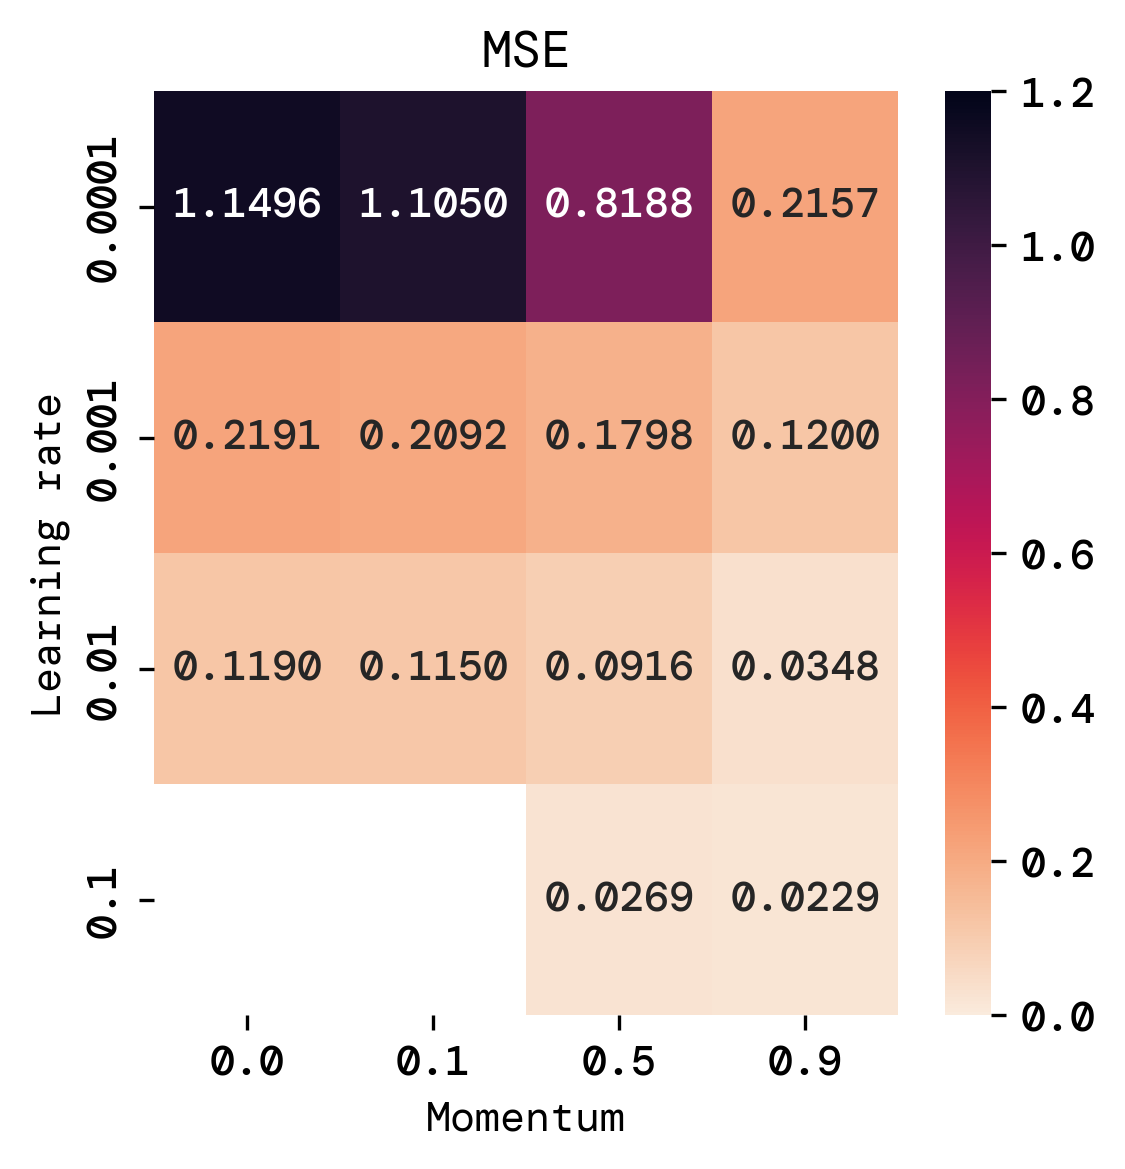
\includegraphics[width=\textwidth]{../runsAndFigures/MSE_lr_gamma.png}
        \end{center}
        \caption{In this case havving momentum seems to be beneficial. We maxes out our testing range and found that 0.9 was the best value for momentum. momentum allows a higher learning rate}\label{fig:MSE_lr_gamma}
    \end{minipage}
    \hspace{1mm}
    \begin{minipage}[t]{0.49\textwidth}
        \begin{center}
            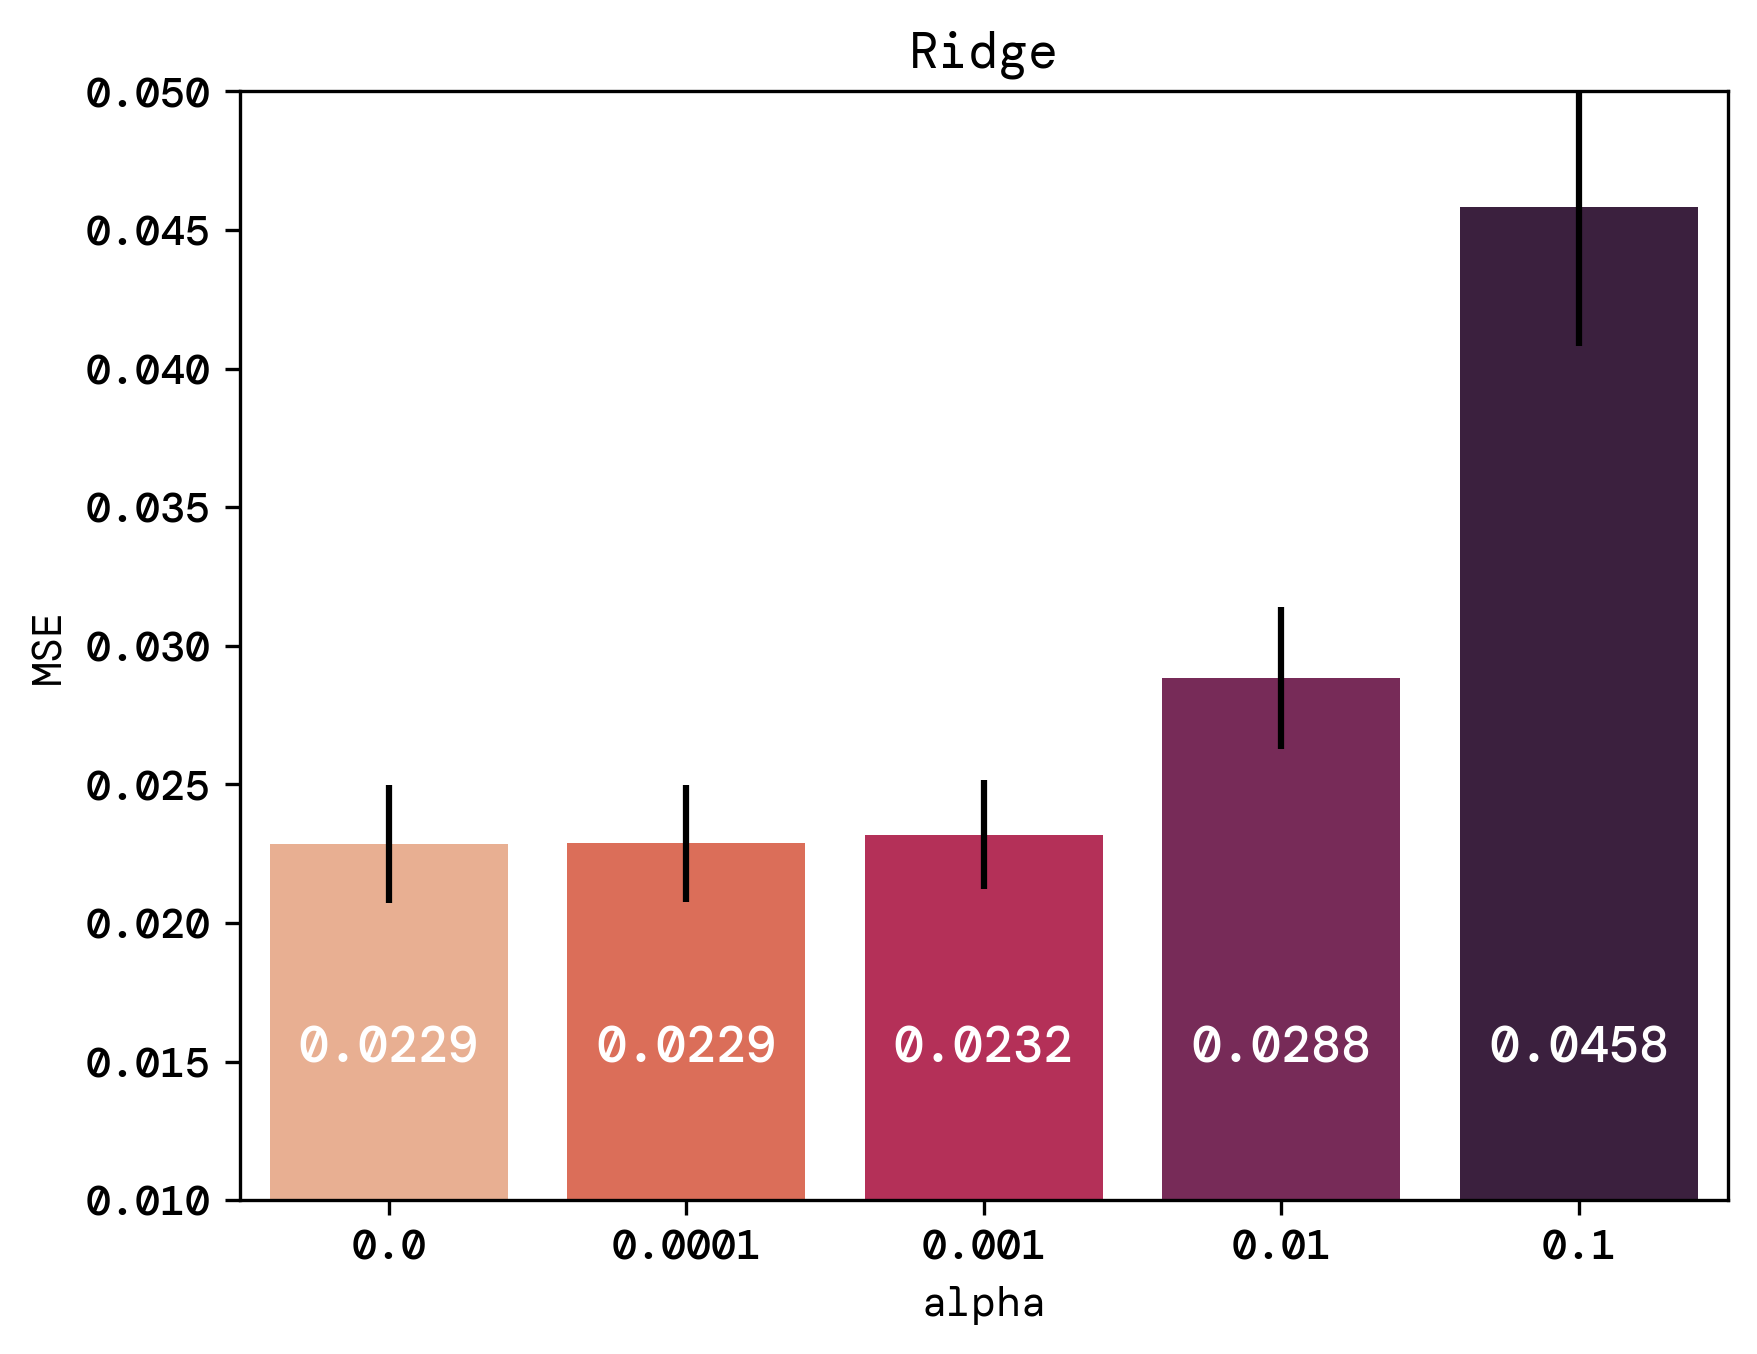
\includegraphics[width=\textwidth]{../runsAndFigures/MSE_alpha.png}
        \end{center}
        \caption{Introduction regualarization does not seem to yield any benefits, in fact
        having too much regualarization shunts performance}\label{fig:MSE_aplha}
    \end{minipage}
\end{figure}


\begin{figure}[!ht]
    \begin{minipage}[t]{0.49\textwidth}
        \begin{center}
            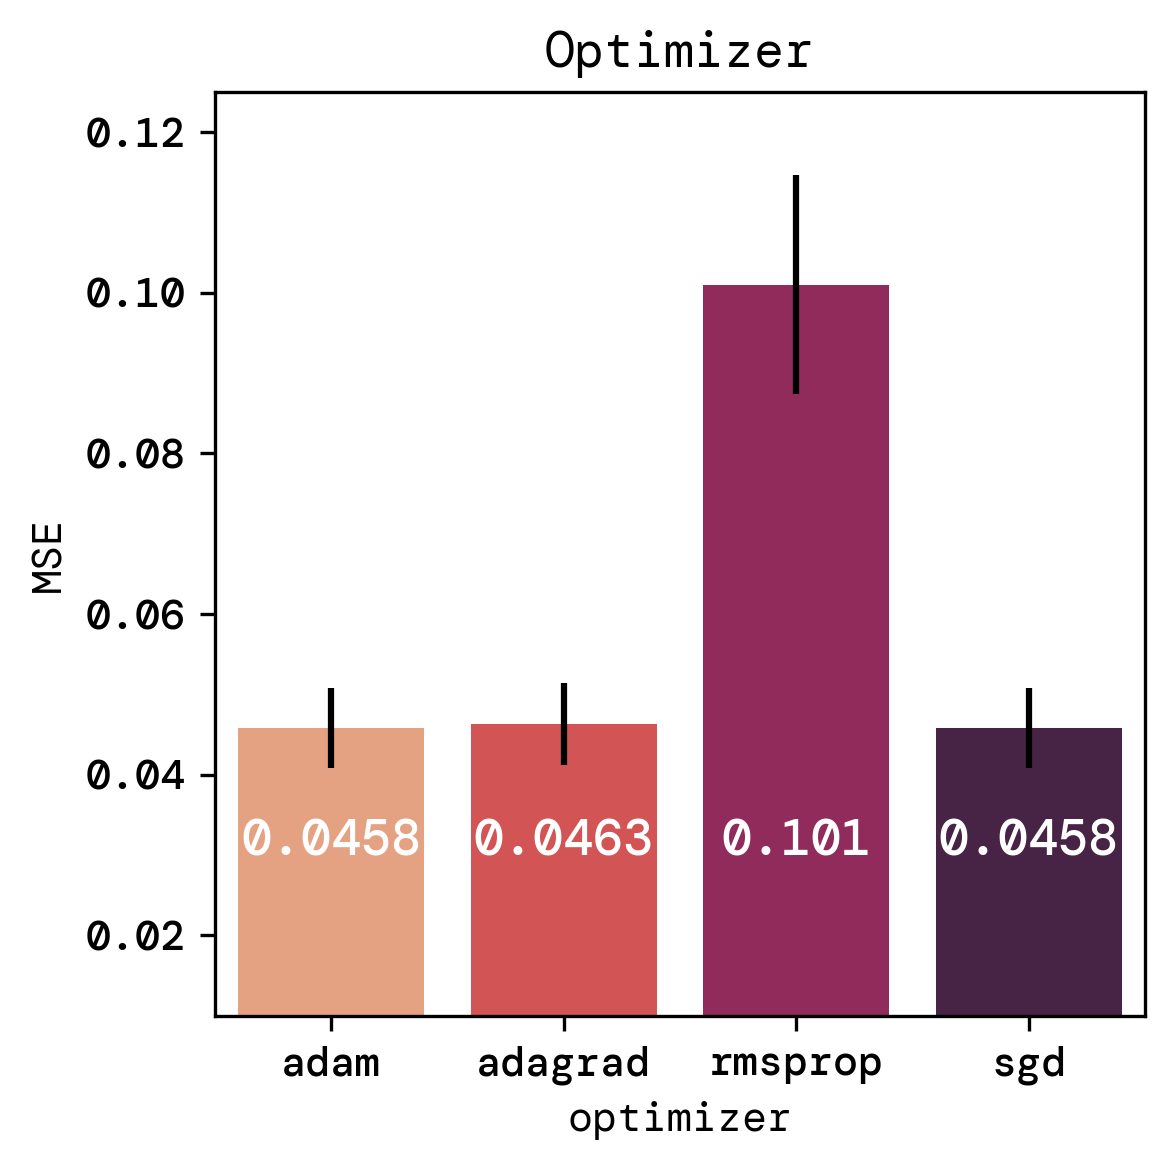
\includegraphics[width=\textwidth]{../runsAndFigures/MSE_optimizer.png}
        \end{center}
        \caption{In this case havving momentum seems to be beneficial. We maxes out our testing range and found that 0.9 was the best value for momentum. momentum allows a higher learning rate}\label{fig:MSE_optimizer}
    \end{minipage}
    \hspace{1mm}
    \begin{minipage}[t]{0.49\textwidth}
        \begin{center}
            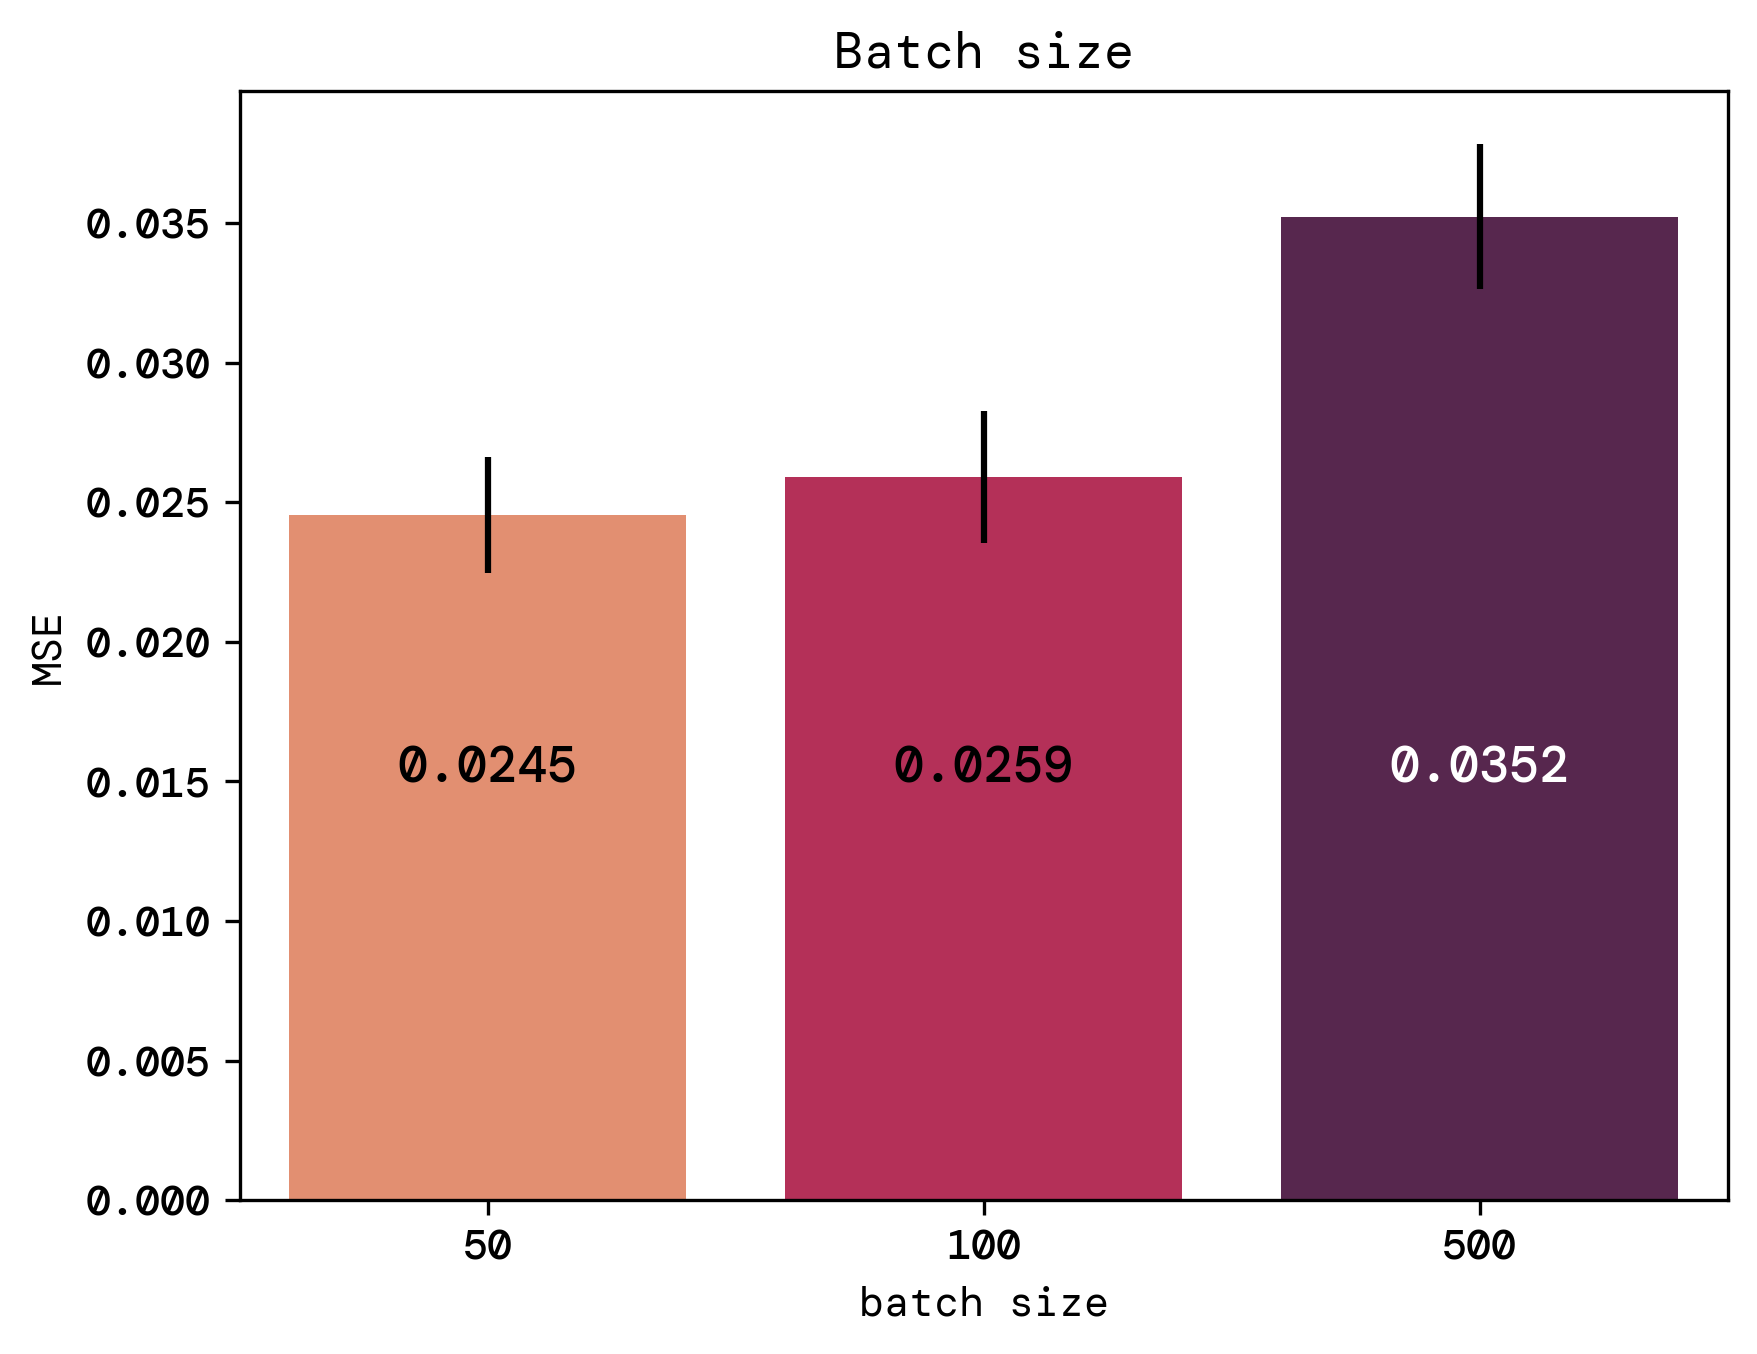
\includegraphics[width=\textwidth]{../runsAndFigures/MSE_batch.png}
        \end{center}
        \caption{Introduction regualarization does not seem to yield any benefits, in fact
        having too much regualarization shunts performance}\label{fig:MSE_batch}
    \end{minipage}
\end{figure}

\begin{figure}[!ht]
    \begin{minipage}[t]{0.5\textwidth - 1mm}
        \begin{center}
            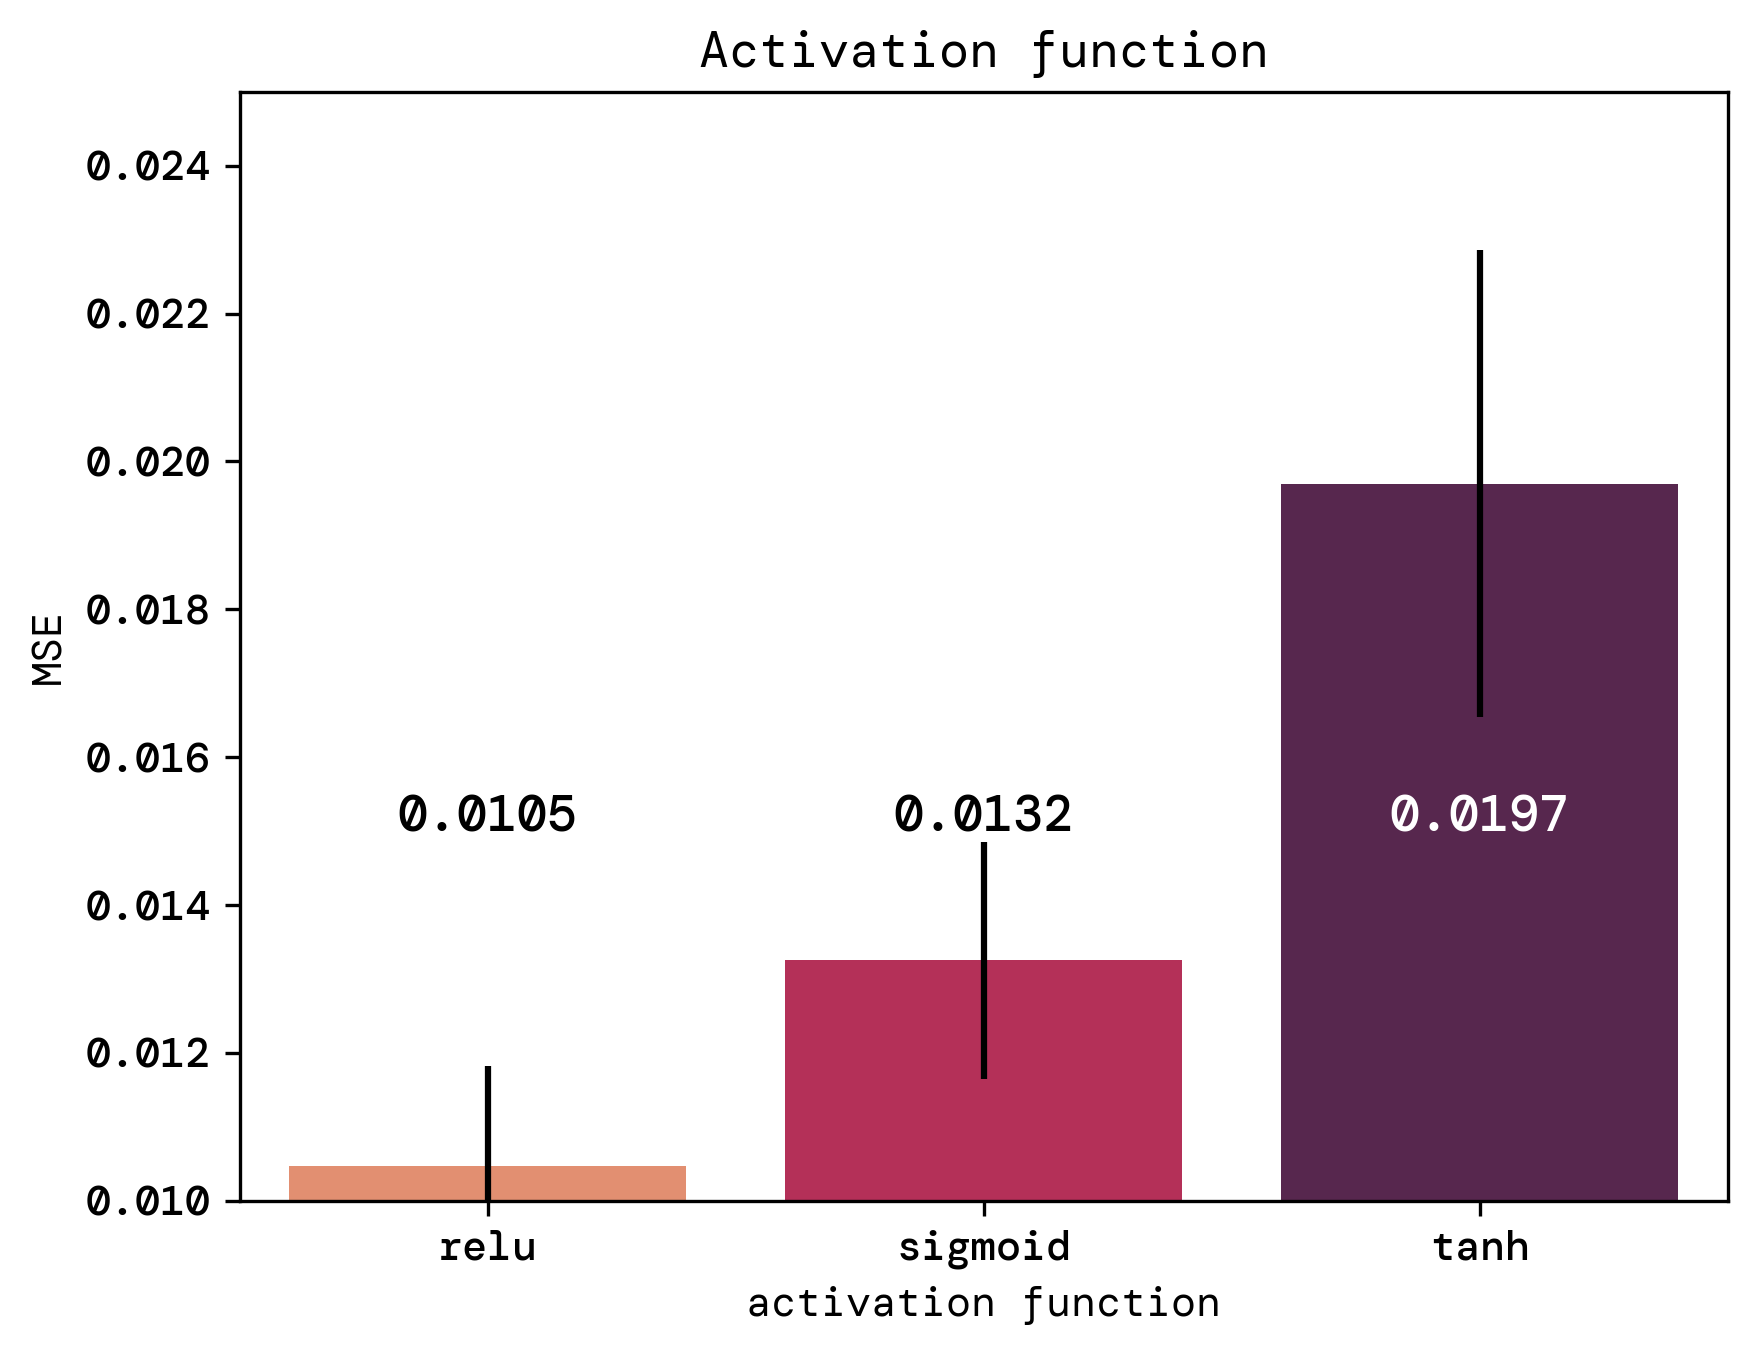
\includegraphics[width=\textwidth]{../runsAndFigures/MSE_activs.png}
        \end{center}
        \caption{In this case havving momentum seems to be beneficial. We maxes out our testing range and found that 0.9 was the best value for momentum. momentum allows a higher learning rate}\label{fig:accuracy_optimizer}
    \end{minipage}
    \hspace{2mm}
    \begin{minipage}[t]{0.5\textwidth - 1mm}
        \begin{center}
            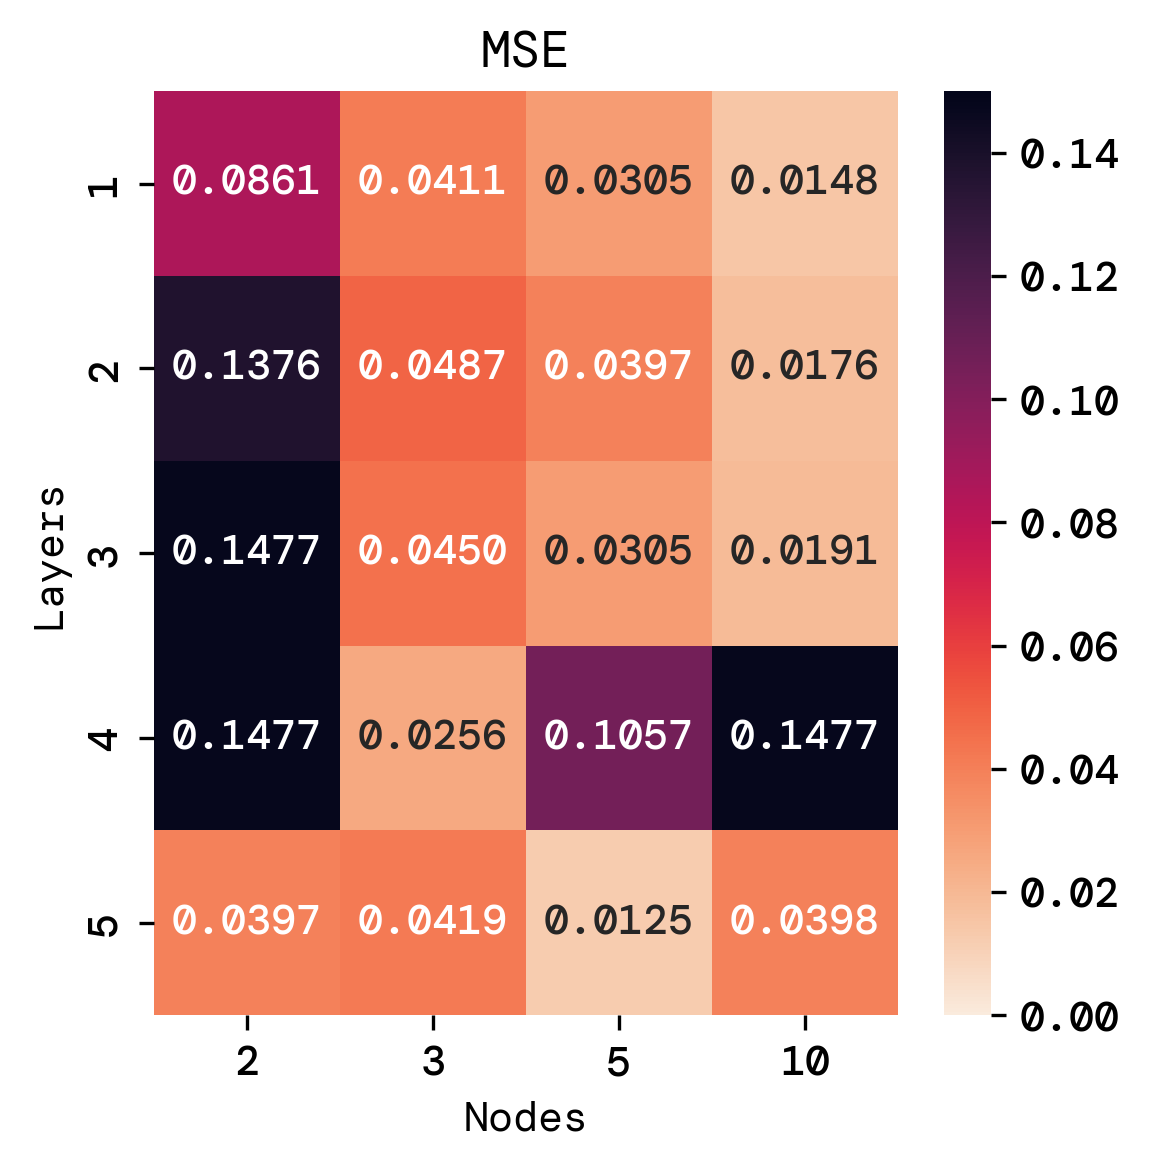
\includegraphics[width=\textwidth]{../runsAndFigures/MSE_layers_nodes.png}
        \end{center}
        \caption{Introduction regualarization does not seem to yield any benefits, in fact
        having too much regualarization shunts performance}\label{fig:accuracy_aplha}
    \end{minipage}
\end{figure}
\subsection*{Final Evaluation and Comparisons}
\label{sec:comparisons2}


















\chapter*{Appendix B}
\label{app:appendix}


\section{Universal Approximation}
\label{sec:UAT}

Where is the limit of what we can learn with a neural network? Can we approximate any function?
There are several ways to approximate a function. For periodic functions it may be wise to use a Fourier series,
another option is to use a Taylor series. If these mehtods don't float your boat, we can in fact use a neural network
instead. A neural network with only one hidden layer can approximate any continuous function
given enough neurons in the hidden layer. The more neurons, the higher the resolution of the Approximation
\cite{HornikEtAl89}. 

\subsection*{XOR VS Perceptron}
\label{app:xor}

A perceptron is a simple model of a neuron. It takes in a set of inputs, multiplies them by a set of weights 
and sums them up to produce an output. The output is then passed through the heaviside
\footnote{We use sigmoid instead of the heaviside, but the outcome of the classification is the same.}
step function to produce
a binary output. The perceptron can be used to solve simple classification problems. However, it is not able to
solve the XOR problem. XOR is not linearly separable, meaning that it is not possible to draw a straight line
that separates the two classes. This is a problem for the perceptron, as it can only draw straight lines.

\begin{figure}[h]
    \begin{center}
        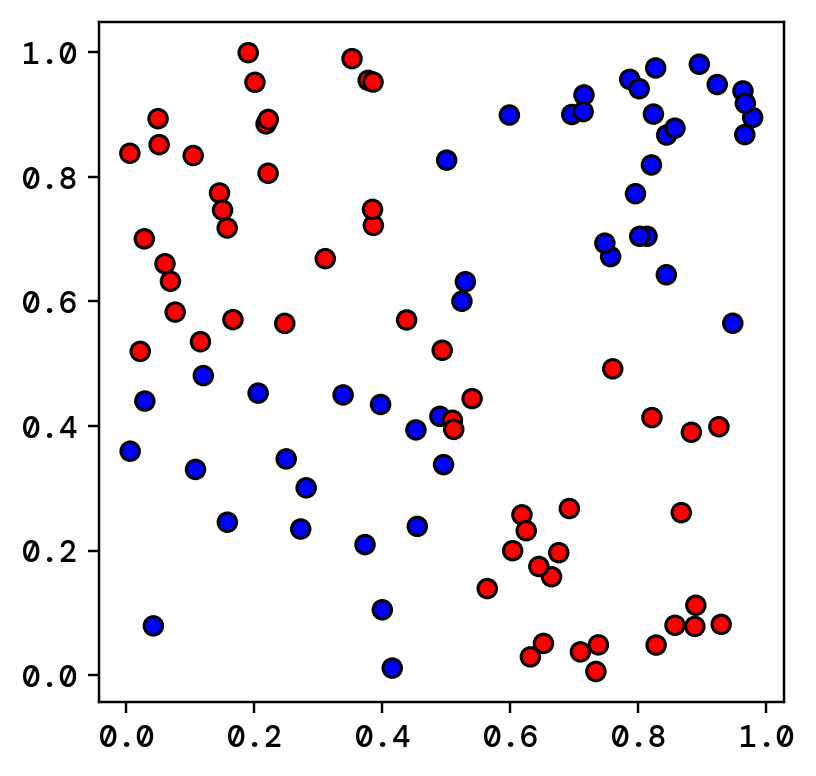
\includegraphics[width=0.5\textwidth]{../runsAndFigures/xor.png}
    \end{center}
    \caption{XOR-variant, it is impossible to separate the two classes with a straight line}\label{fig:xor_data}
\end{figure}


One way to solve this problem is to add some polynomial features to the data. 
This will allow us to draw a curved line that separates the two classes. However, this is not a scalable solution.

\begin{figure}[h]
    \begin{minipage}{0.49\textwidth}
        \begin{center}
            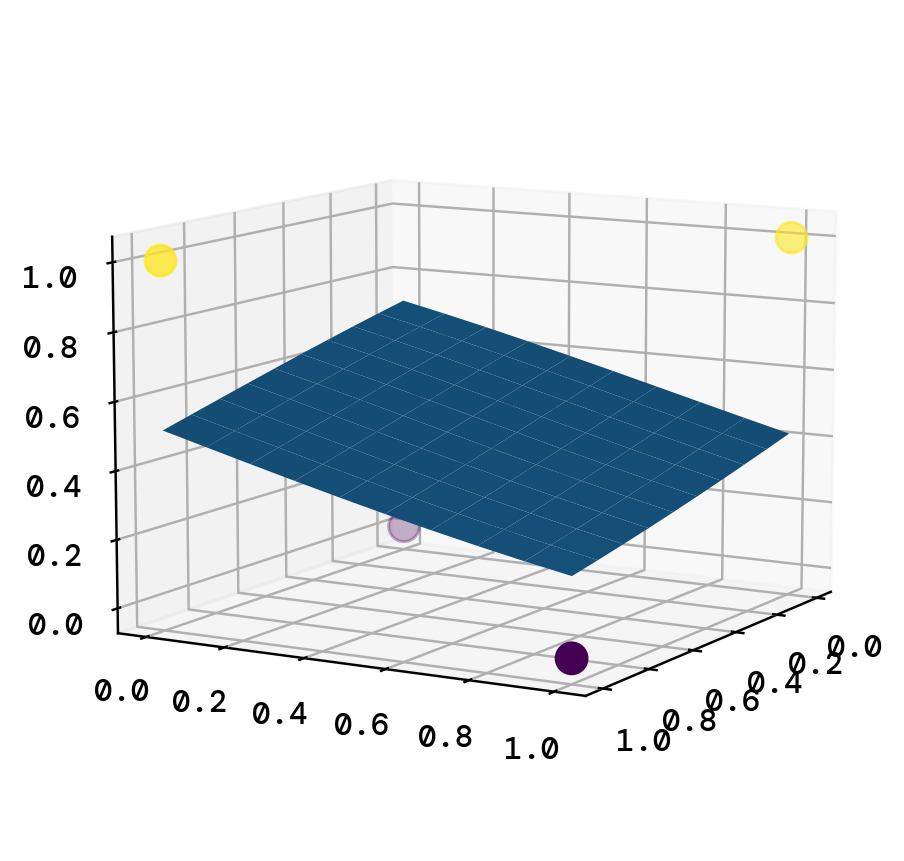
\includegraphics[width=\textwidth]{../runsAndFigures/xor_plain.png}
            \caption{}\label{fig:xor_plain}
        \end{center}
    \end{minipage}
    \hspace{1mm}
    \begin{minipage}{0.49\textwidth}
        \begin{center}
            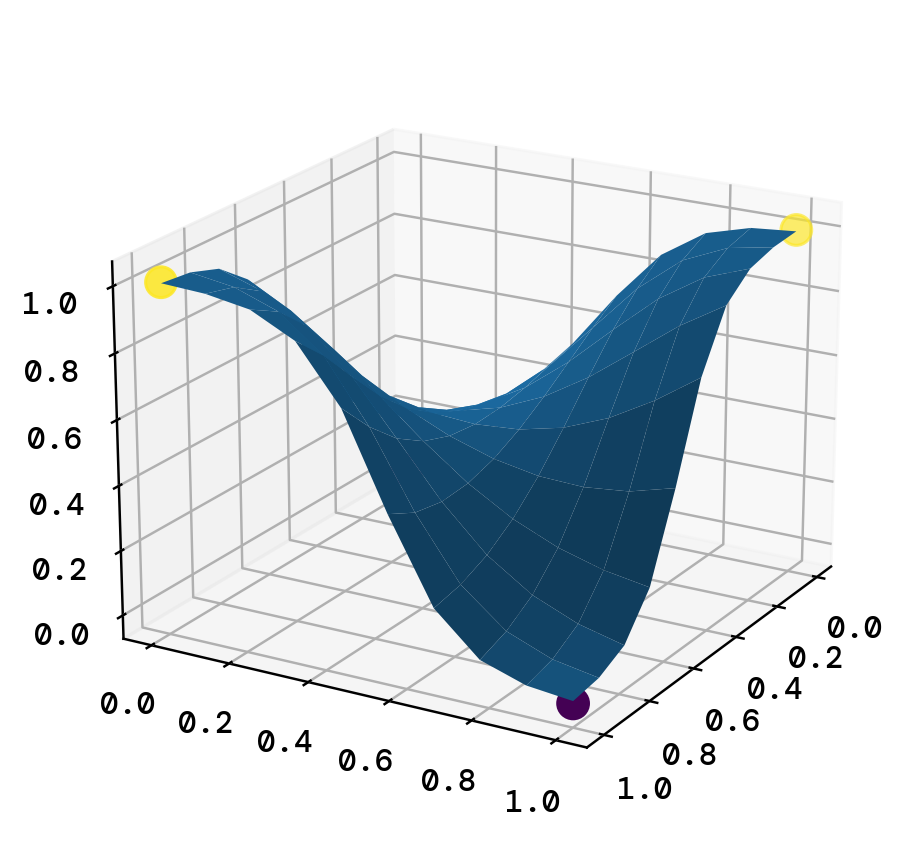
\includegraphics[width=\textwidth]{../runsAndFigures/xor_poly.png}
            \caption{}\label{fig:xor_poly}
        \end{center}
    \end{minipage}
\end{figure}




NNs can also learn xor, without the need for a polynomial feature. This is important because it is not 
always obvious what feature engineering is required to solve a problem. Neural networks can learn the 
relevant 
features from the data. Manually adding polynomial features is not a scalable solution for 
high-dimensional data,
whereas neural networks can learn arbitrarily complex functions. Adding polynomial featurer 
is also prone to 
bias problems.


\begin{figure}[!h]
    \begin{center}
        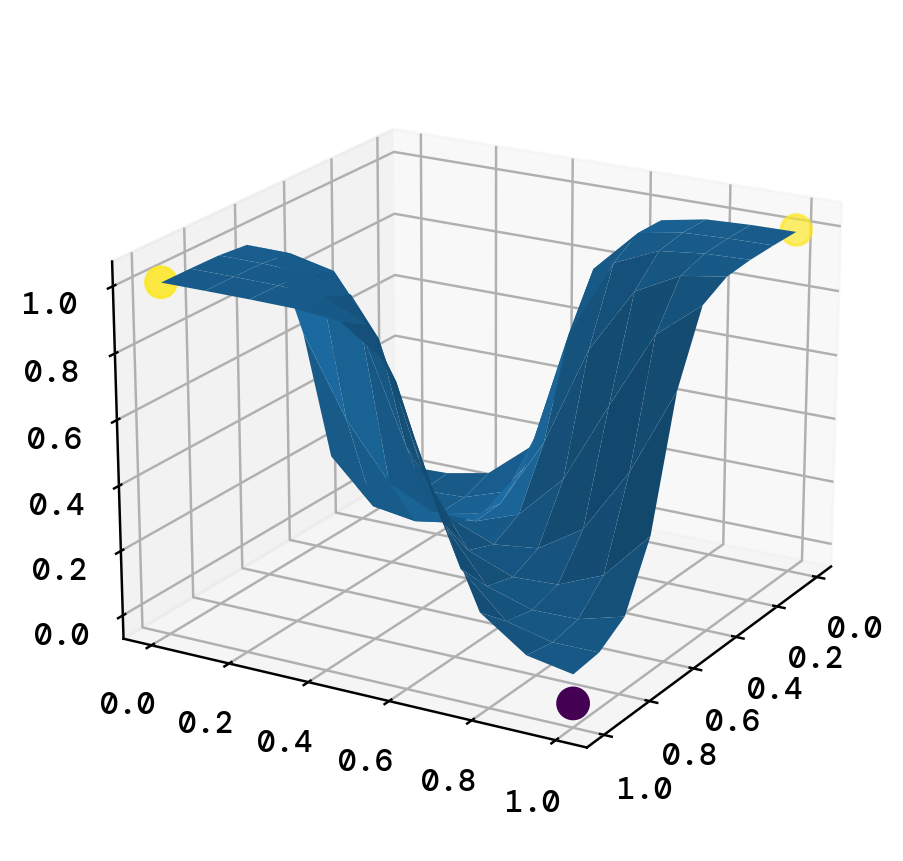
\includegraphics[width=0.5\textwidth]{../runsAndFigures/xor_nn.png}
    \end{center}
    \caption{}\label{fig:xor_nn}
\end{figure}



\subsection*{Combining Neurons}
\label{app:neuronscombined}

We want to approximate this sin function with a neural network. How might that look like?
We can use a single neuron to approximate a line $a w + b$, putting it trough a sigmoid function
we get some non-linearity. Every node in the first hidden layer (and consequents layers) is then 
a line put trough a sigmoid function. The final output of a single hidden layer network is just
a linear combination of these curves. We can add more nodes to get more curves, but we are still


\begin{figure}
    \begin{center}
        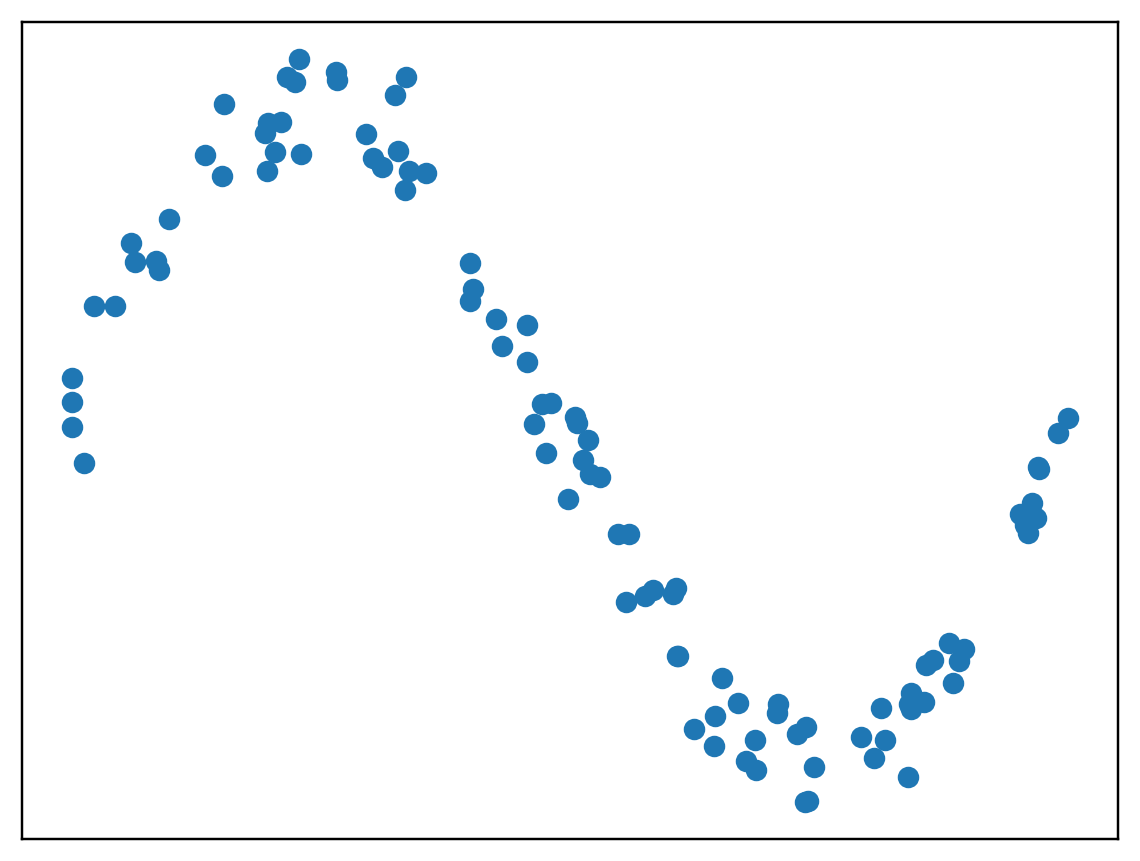
\includegraphics[width=0.4\textwidth]{../runsAndFigures/sin.png}
    \end{center}
    \caption{A $\text{sin}$ function that we want to approximate}\label{fig:sin}
\end{figure}

\begin{figure}
    \begin{center}
        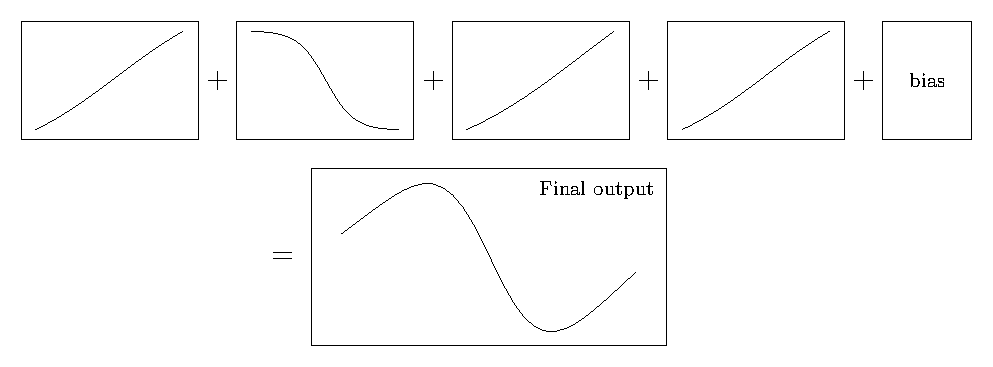
\includegraphics[width=0.95\textwidth]{tikzfigures/universal.pdf}
    \end{center}
    \caption{Four indivudual logistic regression outputs scaled and added together to produce 
    a sin approximation}\label{fig:universal}
\end{figure}


We can chose whatever activation function we want as long as it is non-linear. Relu strugles to learn this 
sin function, but sigmoid works fine.


% \phantomsection%
% \addcontentsline{toc}{subsection}{SVD}
% \subsection*{SVD}
% \label{app:svd}




% \phantomsection%
% \addcontentsline{toc}{subsection}{Confidence Interval}
% \subsection*{Math Behind the Confidence Interval, Section~\ref{sec:confidenceinterval}}
% \label{app:confidenceinterval}




\vskip 0.2in
\bibliography{report}
% \bibliographystyle{apalike}
\bibliographystyle{plain}
% \phantomsection%
\addcontentsline{toc}{section}{Bibliography}
\end{document}








